\documentclass{article}
\usepackage[final]{neurips_2025}  % NEURIPS style (neurips_2025.sty is in paper_draft/)
% neurips_2025.sty leaves \@trackname undefined unless a track option is given;
% define it empty so the footer makes no venue claim.
\makeatletter\providecommand{\@trackname}{}\makeatother
\usepackage[hidelinks]{hyperref}  % REQUIRED: clickable links
\usepackage{booktabs}  % REQUIRED: professional tables
\usepackage{graphicx}
\usepackage{amsmath,amssymb}
\usepackage[utf8]{inputenc}
\usepackage[T1]{fontenc}
\usepackage{enumitem}
\usepackage{caption}
\usepackage{algorithm}
\usepackage[noend]{algpseudocode}

% Import command files
%%%%% MATH NOTATION MACROS %%%%%
% Standard math notation for academic papers
% Import with: %%%%% MATH NOTATION MACROS %%%%%
% Standard math notation for academic papers
% Import with: %%%%% MATH NOTATION MACROS %%%%%
% Standard math notation for academic papers
% Import with: \input{commands/math}

\usepackage{amsmath,amsfonts,bm}

%%%%%%%%%%%%%%%%%%%%%%%%%%%%%%%%%%%%%%%%%%%%%%%%%%%%%%%%%%%%%%%%%
% FIGURE AND SECTION REFERENCES
%%%%%%%%%%%%%%%%%%%%%%%%%%%%%%%%%%%%%%%%%%%%%%%%%%%%%%%%%%%%%%%%%

% Mark sections of captions for referring to divisions of figures
\newcommand{\figleft}{{\em (Left)}}
\newcommand{\figcenter}{{\em (Center)}}
\newcommand{\figright}{{\em (Right)}}
\newcommand{\figtop}{{\em (Top)}}
\newcommand{\figbottom}{{\em (Bottom)}}
\newcommand{\captiona}{{\em (a)}}
\newcommand{\captionb}{{\em (b)}}
\newcommand{\captionc}{{\em (c)}}
\newcommand{\captiond}{{\em (d)}}

% Figure references
\def\figref#1{figure~\ref{#1}}
\def\Figref#1{Figure~\ref{#1}}
\def\twofigref#1#2{figures \ref{#1} and \ref{#2}}
\def\quadfigref#1#2#3#4{figures \ref{#1}, \ref{#2}, \ref{#3} and \ref{#4}}

% Section references
\def\secref#1{section~\ref{#1}}
\def\Secref#1{Section~\ref{#1}}
\def\twosecrefs#1#2{sections \ref{#1} and \ref{#2}}
\def\secrefs#1#2#3{sections \ref{#1}, \ref{#2} and \ref{#3}}

% Equation references
\def\eqref#1{equation~\ref{#1}}
\def\Eqref#1{Equation~\ref{#1}}
\def\plaineqref#1{\ref{#1}}

% Algorithm references
\def\algref#1{algorithm~\ref{#1}}
\def\Algref#1{Algorithm~\ref{#1}}
\def\twoalgref#1#2{algorithms \ref{#1} and \ref{#2}}
\def\Twoalgref#1#2{Algorithms \ref{#1} and \ref{#2}}

% Table references
\def\tabref#1{table~\ref{#1}}
\def\Tabref#1{Table~\ref{#1}}

% Chapter references
\def\chapref#1{chapter~\ref{#1}}
\def\Chapref#1{Chapter~\ref{#1}}

%%%%%%%%%%%%%%%%%%%%%%%%%%%%%%%%%%%%%%%%%%%%%%%%%%%%%%%%%%%%%%%%%
% BASIC MATH DEFINITIONS
%%%%%%%%%%%%%%%%%%%%%%%%%%%%%%%%%%%%%%%%%%%%%%%%%%%%%%%%%%%%%%%%%

\def\ceil#1{\lceil #1 \rceil}
\def\floor#1{\lfloor #1 \rfloor}
\def\1{\bm{1}}
\def\eps{{\epsilon}}

% Common operators
\DeclareMathOperator*{\argmax}{arg\,max}
\DeclareMathOperator*{\argmin}{arg\,min}
\DeclareMathOperator{\sign}{sign}
\DeclareMathOperator{\Tr}{Tr}
\let\ab\allowbreak

%%%%%%%%%%%%%%%%%%%%%%%%%%%%%%%%%%%%%%%%%%%%%%%%%%%%%%%%%%%%%%%%%
% VECTORS (lowercase bold)
%%%%%%%%%%%%%%%%%%%%%%%%%%%%%%%%%%%%%%%%%%%%%%%%%%%%%%%%%%%%%%%%%

\def\vzero{{\bm{0}}}
\def\vone{{\bm{1}}}
\def\vmu{{\bm{\mu}}}
\def\vtheta{{\bm{\theta}}}
\def\va{{\bm{a}}}
\def\vb{{\bm{b}}}
\def\vc{{\bm{c}}}
\def\vd{{\bm{d}}}
\def\ve{{\bm{e}}}
\def\vf{{\bm{f}}}
\def\vg{{\bm{g}}}
\def\vh{{\bm{h}}}
\def\vi{{\bm{i}}}
\def\vj{{\bm{j}}}
\def\vk{{\bm{k}}}
\def\vl{{\bm{l}}}
\def\vm{{\bm{m}}}
\def\vn{{\bm{n}}}
\def\vo{{\bm{o}}}
\def\vp{{\bm{p}}}
\def\vq{{\bm{q}}}
\def\vr{{\bm{r}}}
\def\vs{{\bm{s}}}
\def\vt{{\bm{t}}}
\def\vu{{\bm{u}}}
\def\vv{{\bm{v}}}
\def\vw{{\bm{w}}}
\def\vx{{\bm{x}}}
\def\vy{{\bm{y}}}
\def\vz{{\bm{z}}}

%%%%%%%%%%%%%%%%%%%%%%%%%%%%%%%%%%%%%%%%%%%%%%%%%%%%%%%%%%%%%%%%%
% MATRICES (uppercase bold)
%%%%%%%%%%%%%%%%%%%%%%%%%%%%%%%%%%%%%%%%%%%%%%%%%%%%%%%%%%%%%%%%%

\def\mA{{\bm{A}}}
\def\mB{{\bm{B}}}
\def\mC{{\bm{C}}}
\def\mD{{\bm{D}}}
\def\mE{{\bm{E}}}
\def\mF{{\bm{F}}}
\def\mG{{\bm{G}}}
\def\mH{{\bm{H}}}
\def\mI{{\bm{I}}}
\def\mJ{{\bm{J}}}
\def\mK{{\bm{K}}}
\def\mL{{\bm{L}}}
\def\mM{{\bm{M}}}
\def\mN{{\bm{N}}}
\def\mO{{\bm{O}}}
\def\mP{{\bm{P}}}
\def\mQ{{\bm{Q}}}
\def\mR{{\bm{R}}}
\def\mS{{\bm{S}}}
\def\mT{{\bm{T}}}
\def\mU{{\bm{U}}}
\def\mV{{\bm{V}}}
\def\mW{{\bm{W}}}
\def\mX{{\bm{X}}}
\def\mY{{\bm{Y}}}
\def\mZ{{\bm{Z}}}
\def\mBeta{{\bm{\beta}}}
\def\mPhi{{\bm{\Phi}}}
\def\mLambda{{\bm{\Lambda}}}
\def\mSigma{{\bm{\Sigma}}}

%%%%%%%%%%%%%%%%%%%%%%%%%%%%%%%%%%%%%%%%%%%%%%%%%%%%%%%%%%%%%%%%%
% CALLIGRAPHIC (mathcal)
%%%%%%%%%%%%%%%%%%%%%%%%%%%%%%%%%%%%%%%%%%%%%%%%%%%%%%%%%%%%%%%%%

\def\gA{{\mathcal{A}}}
\def\gB{{\mathcal{B}}}
\def\gC{{\mathcal{C}}}
\def\gD{{\mathcal{D}}}
\def\gE{{\mathcal{E}}}
\def\gF{{\mathcal{F}}}
\def\gG{{\mathcal{G}}}
\def\gH{{\mathcal{H}}}
\def\gI{{\mathcal{I}}}
\def\gJ{{\mathcal{J}}}
\def\gK{{\mathcal{K}}}
\def\gL{{\mathcal{L}}}
\def\gM{{\mathcal{M}}}
\def\gN{{\mathcal{N}}}
\def\gO{{\mathcal{O}}}
\def\gP{{\mathcal{P}}}
\def\gQ{{\mathcal{Q}}}
\def\gR{{\mathcal{R}}}
\def\gS{{\mathcal{S}}}
\def\gT{{\mathcal{T}}}
\def\gU{{\mathcal{U}}}
\def\gV{{\mathcal{V}}}
\def\gW{{\mathcal{W}}}
\def\gX{{\mathcal{X}}}
\def\gY{{\mathcal{Y}}}
\def\gZ{{\mathcal{Z}}}

%%%%%%%%%%%%%%%%%%%%%%%%%%%%%%%%%%%%%%%%%%%%%%%%%%%%%%%%%%%%%%%%%
% SETS (blackboard bold)
%%%%%%%%%%%%%%%%%%%%%%%%%%%%%%%%%%%%%%%%%%%%%%%%%%%%%%%%%%%%%%%%%

\def\sA{{\mathbb{A}}}
\def\sB{{\mathbb{B}}}
\def\sC{{\mathbb{C}}}
\def\sD{{\mathbb{D}}}
\def\sF{{\mathbb{F}}}
\def\sG{{\mathbb{G}}}
\def\sH{{\mathbb{H}}}
\def\sI{{\mathbb{I}}}
\def\sJ{{\mathbb{J}}}
\def\sK{{\mathbb{K}}}
\def\sL{{\mathbb{L}}}
\def\sM{{\mathbb{M}}}
\def\sN{{\mathbb{N}}}
\def\sO{{\mathbb{O}}}
\def\sP{{\mathbb{P}}}
\def\sQ{{\mathbb{Q}}}
\def\sR{{\mathbb{R}}}
\def\sS{{\mathbb{S}}}
\def\sT{{\mathbb{T}}}
\def\sU{{\mathbb{U}}}
\def\sV{{\mathbb{V}}}
\def\sW{{\mathbb{W}}}
\def\sX{{\mathbb{X}}}
\def\sY{{\mathbb{Y}}}
\def\sZ{{\mathbb{Z}}}

%%%%%%%%%%%%%%%%%%%%%%%%%%%%%%%%%%%%%%%%%%%%%%%%%%%%%%%%%%%%%%%%%
% COMMON MATH SHORTCUTS
%%%%%%%%%%%%%%%%%%%%%%%%%%%%%%%%%%%%%%%%%%%%%%%%%%%%%%%%%%%%%%%%%

% Expectation and variance
\newcommand{\E}{\mathbb{E}}
\newcommand{\Var}{\mathrm{Var}}
\newcommand{\Cov}{\mathrm{Cov}}
\newcommand{\R}{\mathbb{R}}

% Datasets
\newcommand{\train}{\mathcal{D}}
\newcommand{\valid}{\mathcal{D_{\mathrm{valid}}}}
\newcommand{\test}{\mathcal{D_{\mathrm{test}}}}

% Distributions
\newcommand{\laplace}{\mathrm{Laplace}}
\newcommand{\Uniform}{\mathrm{Unif}}
\newcommand{\Normal}{\mathrm{Normal}}
\newcommand{\Categorical}{\mathrm{Categorical}}

% Common functions
\newcommand{\softmax}{\mathrm{softmax}}
\newcommand{\sigmoid}{\sigma}
\newcommand{\KL}{D_{\mathrm{KL}}}

% Norms
\newcommand{\normlzero}{L^0}
\newcommand{\normlone}{L^1}
\newcommand{\normltwo}{L^2}
\newcommand{\normlp}{L^p}
\newcommand{\normmax}{L^\infty}

%%%%%%%%%%%%%%%%%%%%%%%%%%%%%%%%%%%%%%%%%%%%%%%%%%%%%%%%%%%%%%%%%
% DEFINITIONS AND HIGHLIGHTING
%%%%%%%%%%%%%%%%%%%%%%%%%%%%%%%%%%%%%%%%%%%%%%%%%%%%%%%%%%%%%%%%%

% Highlight a newly defined term
\newcommand{\newterm}[1]{{\bf #1}}
\newcommand{\defn}[1]{\textbf{#1}}
\newcommand{\defeq}{\mathrel{\stackrel{\textnormal{\tiny def}}{=}}}


\usepackage{amsmath,amsfonts,bm}

%%%%%%%%%%%%%%%%%%%%%%%%%%%%%%%%%%%%%%%%%%%%%%%%%%%%%%%%%%%%%%%%%
% FIGURE AND SECTION REFERENCES
%%%%%%%%%%%%%%%%%%%%%%%%%%%%%%%%%%%%%%%%%%%%%%%%%%%%%%%%%%%%%%%%%

% Mark sections of captions for referring to divisions of figures
\newcommand{\figleft}{{\em (Left)}}
\newcommand{\figcenter}{{\em (Center)}}
\newcommand{\figright}{{\em (Right)}}
\newcommand{\figtop}{{\em (Top)}}
\newcommand{\figbottom}{{\em (Bottom)}}
\newcommand{\captiona}{{\em (a)}}
\newcommand{\captionb}{{\em (b)}}
\newcommand{\captionc}{{\em (c)}}
\newcommand{\captiond}{{\em (d)}}

% Figure references
\def\figref#1{figure~\ref{#1}}
\def\Figref#1{Figure~\ref{#1}}
\def\twofigref#1#2{figures \ref{#1} and \ref{#2}}
\def\quadfigref#1#2#3#4{figures \ref{#1}, \ref{#2}, \ref{#3} and \ref{#4}}

% Section references
\def\secref#1{section~\ref{#1}}
\def\Secref#1{Section~\ref{#1}}
\def\twosecrefs#1#2{sections \ref{#1} and \ref{#2}}
\def\secrefs#1#2#3{sections \ref{#1}, \ref{#2} and \ref{#3}}

% Equation references
\def\eqref#1{equation~\ref{#1}}
\def\Eqref#1{Equation~\ref{#1}}
\def\plaineqref#1{\ref{#1}}

% Algorithm references
\def\algref#1{algorithm~\ref{#1}}
\def\Algref#1{Algorithm~\ref{#1}}
\def\twoalgref#1#2{algorithms \ref{#1} and \ref{#2}}
\def\Twoalgref#1#2{Algorithms \ref{#1} and \ref{#2}}

% Table references
\def\tabref#1{table~\ref{#1}}
\def\Tabref#1{Table~\ref{#1}}

% Chapter references
\def\chapref#1{chapter~\ref{#1}}
\def\Chapref#1{Chapter~\ref{#1}}

%%%%%%%%%%%%%%%%%%%%%%%%%%%%%%%%%%%%%%%%%%%%%%%%%%%%%%%%%%%%%%%%%
% BASIC MATH DEFINITIONS
%%%%%%%%%%%%%%%%%%%%%%%%%%%%%%%%%%%%%%%%%%%%%%%%%%%%%%%%%%%%%%%%%

\def\ceil#1{\lceil #1 \rceil}
\def\floor#1{\lfloor #1 \rfloor}
\def\1{\bm{1}}
\def\eps{{\epsilon}}

% Common operators
\DeclareMathOperator*{\argmax}{arg\,max}
\DeclareMathOperator*{\argmin}{arg\,min}
\DeclareMathOperator{\sign}{sign}
\DeclareMathOperator{\Tr}{Tr}
\let\ab\allowbreak

%%%%%%%%%%%%%%%%%%%%%%%%%%%%%%%%%%%%%%%%%%%%%%%%%%%%%%%%%%%%%%%%%
% VECTORS (lowercase bold)
%%%%%%%%%%%%%%%%%%%%%%%%%%%%%%%%%%%%%%%%%%%%%%%%%%%%%%%%%%%%%%%%%

\def\vzero{{\bm{0}}}
\def\vone{{\bm{1}}}
\def\vmu{{\bm{\mu}}}
\def\vtheta{{\bm{\theta}}}
\def\va{{\bm{a}}}
\def\vb{{\bm{b}}}
\def\vc{{\bm{c}}}
\def\vd{{\bm{d}}}
\def\ve{{\bm{e}}}
\def\vf{{\bm{f}}}
\def\vg{{\bm{g}}}
\def\vh{{\bm{h}}}
\def\vi{{\bm{i}}}
\def\vj{{\bm{j}}}
\def\vk{{\bm{k}}}
\def\vl{{\bm{l}}}
\def\vm{{\bm{m}}}
\def\vn{{\bm{n}}}
\def\vo{{\bm{o}}}
\def\vp{{\bm{p}}}
\def\vq{{\bm{q}}}
\def\vr{{\bm{r}}}
\def\vs{{\bm{s}}}
\def\vt{{\bm{t}}}
\def\vu{{\bm{u}}}
\def\vv{{\bm{v}}}
\def\vw{{\bm{w}}}
\def\vx{{\bm{x}}}
\def\vy{{\bm{y}}}
\def\vz{{\bm{z}}}

%%%%%%%%%%%%%%%%%%%%%%%%%%%%%%%%%%%%%%%%%%%%%%%%%%%%%%%%%%%%%%%%%
% MATRICES (uppercase bold)
%%%%%%%%%%%%%%%%%%%%%%%%%%%%%%%%%%%%%%%%%%%%%%%%%%%%%%%%%%%%%%%%%

\def\mA{{\bm{A}}}
\def\mB{{\bm{B}}}
\def\mC{{\bm{C}}}
\def\mD{{\bm{D}}}
\def\mE{{\bm{E}}}
\def\mF{{\bm{F}}}
\def\mG{{\bm{G}}}
\def\mH{{\bm{H}}}
\def\mI{{\bm{I}}}
\def\mJ{{\bm{J}}}
\def\mK{{\bm{K}}}
\def\mL{{\bm{L}}}
\def\mM{{\bm{M}}}
\def\mN{{\bm{N}}}
\def\mO{{\bm{O}}}
\def\mP{{\bm{P}}}
\def\mQ{{\bm{Q}}}
\def\mR{{\bm{R}}}
\def\mS{{\bm{S}}}
\def\mT{{\bm{T}}}
\def\mU{{\bm{U}}}
\def\mV{{\bm{V}}}
\def\mW{{\bm{W}}}
\def\mX{{\bm{X}}}
\def\mY{{\bm{Y}}}
\def\mZ{{\bm{Z}}}
\def\mBeta{{\bm{\beta}}}
\def\mPhi{{\bm{\Phi}}}
\def\mLambda{{\bm{\Lambda}}}
\def\mSigma{{\bm{\Sigma}}}

%%%%%%%%%%%%%%%%%%%%%%%%%%%%%%%%%%%%%%%%%%%%%%%%%%%%%%%%%%%%%%%%%
% CALLIGRAPHIC (mathcal)
%%%%%%%%%%%%%%%%%%%%%%%%%%%%%%%%%%%%%%%%%%%%%%%%%%%%%%%%%%%%%%%%%

\def\gA{{\mathcal{A}}}
\def\gB{{\mathcal{B}}}
\def\gC{{\mathcal{C}}}
\def\gD{{\mathcal{D}}}
\def\gE{{\mathcal{E}}}
\def\gF{{\mathcal{F}}}
\def\gG{{\mathcal{G}}}
\def\gH{{\mathcal{H}}}
\def\gI{{\mathcal{I}}}
\def\gJ{{\mathcal{J}}}
\def\gK{{\mathcal{K}}}
\def\gL{{\mathcal{L}}}
\def\gM{{\mathcal{M}}}
\def\gN{{\mathcal{N}}}
\def\gO{{\mathcal{O}}}
\def\gP{{\mathcal{P}}}
\def\gQ{{\mathcal{Q}}}
\def\gR{{\mathcal{R}}}
\def\gS{{\mathcal{S}}}
\def\gT{{\mathcal{T}}}
\def\gU{{\mathcal{U}}}
\def\gV{{\mathcal{V}}}
\def\gW{{\mathcal{W}}}
\def\gX{{\mathcal{X}}}
\def\gY{{\mathcal{Y}}}
\def\gZ{{\mathcal{Z}}}

%%%%%%%%%%%%%%%%%%%%%%%%%%%%%%%%%%%%%%%%%%%%%%%%%%%%%%%%%%%%%%%%%
% SETS (blackboard bold)
%%%%%%%%%%%%%%%%%%%%%%%%%%%%%%%%%%%%%%%%%%%%%%%%%%%%%%%%%%%%%%%%%

\def\sA{{\mathbb{A}}}
\def\sB{{\mathbb{B}}}
\def\sC{{\mathbb{C}}}
\def\sD{{\mathbb{D}}}
\def\sF{{\mathbb{F}}}
\def\sG{{\mathbb{G}}}
\def\sH{{\mathbb{H}}}
\def\sI{{\mathbb{I}}}
\def\sJ{{\mathbb{J}}}
\def\sK{{\mathbb{K}}}
\def\sL{{\mathbb{L}}}
\def\sM{{\mathbb{M}}}
\def\sN{{\mathbb{N}}}
\def\sO{{\mathbb{O}}}
\def\sP{{\mathbb{P}}}
\def\sQ{{\mathbb{Q}}}
\def\sR{{\mathbb{R}}}
\def\sS{{\mathbb{S}}}
\def\sT{{\mathbb{T}}}
\def\sU{{\mathbb{U}}}
\def\sV{{\mathbb{V}}}
\def\sW{{\mathbb{W}}}
\def\sX{{\mathbb{X}}}
\def\sY{{\mathbb{Y}}}
\def\sZ{{\mathbb{Z}}}

%%%%%%%%%%%%%%%%%%%%%%%%%%%%%%%%%%%%%%%%%%%%%%%%%%%%%%%%%%%%%%%%%
% COMMON MATH SHORTCUTS
%%%%%%%%%%%%%%%%%%%%%%%%%%%%%%%%%%%%%%%%%%%%%%%%%%%%%%%%%%%%%%%%%

% Expectation and variance
\newcommand{\E}{\mathbb{E}}
\newcommand{\Var}{\mathrm{Var}}
\newcommand{\Cov}{\mathrm{Cov}}
\newcommand{\R}{\mathbb{R}}

% Datasets
\newcommand{\train}{\mathcal{D}}
\newcommand{\valid}{\mathcal{D_{\mathrm{valid}}}}
\newcommand{\test}{\mathcal{D_{\mathrm{test}}}}

% Distributions
\newcommand{\laplace}{\mathrm{Laplace}}
\newcommand{\Uniform}{\mathrm{Unif}}
\newcommand{\Normal}{\mathrm{Normal}}
\newcommand{\Categorical}{\mathrm{Categorical}}

% Common functions
\newcommand{\softmax}{\mathrm{softmax}}
\newcommand{\sigmoid}{\sigma}
\newcommand{\KL}{D_{\mathrm{KL}}}

% Norms
\newcommand{\normlzero}{L^0}
\newcommand{\normlone}{L^1}
\newcommand{\normltwo}{L^2}
\newcommand{\normlp}{L^p}
\newcommand{\normmax}{L^\infty}

%%%%%%%%%%%%%%%%%%%%%%%%%%%%%%%%%%%%%%%%%%%%%%%%%%%%%%%%%%%%%%%%%
% DEFINITIONS AND HIGHLIGHTING
%%%%%%%%%%%%%%%%%%%%%%%%%%%%%%%%%%%%%%%%%%%%%%%%%%%%%%%%%%%%%%%%%

% Highlight a newly defined term
\newcommand{\newterm}[1]{{\bf #1}}
\newcommand{\defn}[1]{\textbf{#1}}
\newcommand{\defeq}{\mathrel{\stackrel{\textnormal{\tiny def}}{=}}}


\usepackage{amsmath,amsfonts,bm}

%%%%%%%%%%%%%%%%%%%%%%%%%%%%%%%%%%%%%%%%%%%%%%%%%%%%%%%%%%%%%%%%%
% FIGURE AND SECTION REFERENCES
%%%%%%%%%%%%%%%%%%%%%%%%%%%%%%%%%%%%%%%%%%%%%%%%%%%%%%%%%%%%%%%%%

% Mark sections of captions for referring to divisions of figures
\newcommand{\figleft}{{\em (Left)}}
\newcommand{\figcenter}{{\em (Center)}}
\newcommand{\figright}{{\em (Right)}}
\newcommand{\figtop}{{\em (Top)}}
\newcommand{\figbottom}{{\em (Bottom)}}
\newcommand{\captiona}{{\em (a)}}
\newcommand{\captionb}{{\em (b)}}
\newcommand{\captionc}{{\em (c)}}
\newcommand{\captiond}{{\em (d)}}

% Figure references
\def\figref#1{figure~\ref{#1}}
\def\Figref#1{Figure~\ref{#1}}
\def\twofigref#1#2{figures \ref{#1} and \ref{#2}}
\def\quadfigref#1#2#3#4{figures \ref{#1}, \ref{#2}, \ref{#3} and \ref{#4}}

% Section references
\def\secref#1{section~\ref{#1}}
\def\Secref#1{Section~\ref{#1}}
\def\twosecrefs#1#2{sections \ref{#1} and \ref{#2}}
\def\secrefs#1#2#3{sections \ref{#1}, \ref{#2} and \ref{#3}}

% Equation references
\def\eqref#1{equation~\ref{#1}}
\def\Eqref#1{Equation~\ref{#1}}
\def\plaineqref#1{\ref{#1}}

% Algorithm references
\def\algref#1{algorithm~\ref{#1}}
\def\Algref#1{Algorithm~\ref{#1}}
\def\twoalgref#1#2{algorithms \ref{#1} and \ref{#2}}
\def\Twoalgref#1#2{Algorithms \ref{#1} and \ref{#2}}

% Table references
\def\tabref#1{table~\ref{#1}}
\def\Tabref#1{Table~\ref{#1}}

% Chapter references
\def\chapref#1{chapter~\ref{#1}}
\def\Chapref#1{Chapter~\ref{#1}}

%%%%%%%%%%%%%%%%%%%%%%%%%%%%%%%%%%%%%%%%%%%%%%%%%%%%%%%%%%%%%%%%%
% BASIC MATH DEFINITIONS
%%%%%%%%%%%%%%%%%%%%%%%%%%%%%%%%%%%%%%%%%%%%%%%%%%%%%%%%%%%%%%%%%

\def\ceil#1{\lceil #1 \rceil}
\def\floor#1{\lfloor #1 \rfloor}
\def\1{\bm{1}}
\def\eps{{\epsilon}}

% Common operators
\DeclareMathOperator*{\argmax}{arg\,max}
\DeclareMathOperator*{\argmin}{arg\,min}
\DeclareMathOperator{\sign}{sign}
\DeclareMathOperator{\Tr}{Tr}
\let\ab\allowbreak

%%%%%%%%%%%%%%%%%%%%%%%%%%%%%%%%%%%%%%%%%%%%%%%%%%%%%%%%%%%%%%%%%
% VECTORS (lowercase bold)
%%%%%%%%%%%%%%%%%%%%%%%%%%%%%%%%%%%%%%%%%%%%%%%%%%%%%%%%%%%%%%%%%

\def\vzero{{\bm{0}}}
\def\vone{{\bm{1}}}
\def\vmu{{\bm{\mu}}}
\def\vtheta{{\bm{\theta}}}
\def\va{{\bm{a}}}
\def\vb{{\bm{b}}}
\def\vc{{\bm{c}}}
\def\vd{{\bm{d}}}
\def\ve{{\bm{e}}}
\def\vf{{\bm{f}}}
\def\vg{{\bm{g}}}
\def\vh{{\bm{h}}}
\def\vi{{\bm{i}}}
\def\vj{{\bm{j}}}
\def\vk{{\bm{k}}}
\def\vl{{\bm{l}}}
\def\vm{{\bm{m}}}
\def\vn{{\bm{n}}}
\def\vo{{\bm{o}}}
\def\vp{{\bm{p}}}
\def\vq{{\bm{q}}}
\def\vr{{\bm{r}}}
\def\vs{{\bm{s}}}
\def\vt{{\bm{t}}}
\def\vu{{\bm{u}}}
\def\vv{{\bm{v}}}
\def\vw{{\bm{w}}}
\def\vx{{\bm{x}}}
\def\vy{{\bm{y}}}
\def\vz{{\bm{z}}}

%%%%%%%%%%%%%%%%%%%%%%%%%%%%%%%%%%%%%%%%%%%%%%%%%%%%%%%%%%%%%%%%%
% MATRICES (uppercase bold)
%%%%%%%%%%%%%%%%%%%%%%%%%%%%%%%%%%%%%%%%%%%%%%%%%%%%%%%%%%%%%%%%%

\def\mA{{\bm{A}}}
\def\mB{{\bm{B}}}
\def\mC{{\bm{C}}}
\def\mD{{\bm{D}}}
\def\mE{{\bm{E}}}
\def\mF{{\bm{F}}}
\def\mG{{\bm{G}}}
\def\mH{{\bm{H}}}
\def\mI{{\bm{I}}}
\def\mJ{{\bm{J}}}
\def\mK{{\bm{K}}}
\def\mL{{\bm{L}}}
\def\mM{{\bm{M}}}
\def\mN{{\bm{N}}}
\def\mO{{\bm{O}}}
\def\mP{{\bm{P}}}
\def\mQ{{\bm{Q}}}
\def\mR{{\bm{R}}}
\def\mS{{\bm{S}}}
\def\mT{{\bm{T}}}
\def\mU{{\bm{U}}}
\def\mV{{\bm{V}}}
\def\mW{{\bm{W}}}
\def\mX{{\bm{X}}}
\def\mY{{\bm{Y}}}
\def\mZ{{\bm{Z}}}
\def\mBeta{{\bm{\beta}}}
\def\mPhi{{\bm{\Phi}}}
\def\mLambda{{\bm{\Lambda}}}
\def\mSigma{{\bm{\Sigma}}}

%%%%%%%%%%%%%%%%%%%%%%%%%%%%%%%%%%%%%%%%%%%%%%%%%%%%%%%%%%%%%%%%%
% CALLIGRAPHIC (mathcal)
%%%%%%%%%%%%%%%%%%%%%%%%%%%%%%%%%%%%%%%%%%%%%%%%%%%%%%%%%%%%%%%%%

\def\gA{{\mathcal{A}}}
\def\gB{{\mathcal{B}}}
\def\gC{{\mathcal{C}}}
\def\gD{{\mathcal{D}}}
\def\gE{{\mathcal{E}}}
\def\gF{{\mathcal{F}}}
\def\gG{{\mathcal{G}}}
\def\gH{{\mathcal{H}}}
\def\gI{{\mathcal{I}}}
\def\gJ{{\mathcal{J}}}
\def\gK{{\mathcal{K}}}
\def\gL{{\mathcal{L}}}
\def\gM{{\mathcal{M}}}
\def\gN{{\mathcal{N}}}
\def\gO{{\mathcal{O}}}
\def\gP{{\mathcal{P}}}
\def\gQ{{\mathcal{Q}}}
\def\gR{{\mathcal{R}}}
\def\gS{{\mathcal{S}}}
\def\gT{{\mathcal{T}}}
\def\gU{{\mathcal{U}}}
\def\gV{{\mathcal{V}}}
\def\gW{{\mathcal{W}}}
\def\gX{{\mathcal{X}}}
\def\gY{{\mathcal{Y}}}
\def\gZ{{\mathcal{Z}}}

%%%%%%%%%%%%%%%%%%%%%%%%%%%%%%%%%%%%%%%%%%%%%%%%%%%%%%%%%%%%%%%%%
% SETS (blackboard bold)
%%%%%%%%%%%%%%%%%%%%%%%%%%%%%%%%%%%%%%%%%%%%%%%%%%%%%%%%%%%%%%%%%

\def\sA{{\mathbb{A}}}
\def\sB{{\mathbb{B}}}
\def\sC{{\mathbb{C}}}
\def\sD{{\mathbb{D}}}
\def\sF{{\mathbb{F}}}
\def\sG{{\mathbb{G}}}
\def\sH{{\mathbb{H}}}
\def\sI{{\mathbb{I}}}
\def\sJ{{\mathbb{J}}}
\def\sK{{\mathbb{K}}}
\def\sL{{\mathbb{L}}}
\def\sM{{\mathbb{M}}}
\def\sN{{\mathbb{N}}}
\def\sO{{\mathbb{O}}}
\def\sP{{\mathbb{P}}}
\def\sQ{{\mathbb{Q}}}
\def\sR{{\mathbb{R}}}
\def\sS{{\mathbb{S}}}
\def\sT{{\mathbb{T}}}
\def\sU{{\mathbb{U}}}
\def\sV{{\mathbb{V}}}
\def\sW{{\mathbb{W}}}
\def\sX{{\mathbb{X}}}
\def\sY{{\mathbb{Y}}}
\def\sZ{{\mathbb{Z}}}

%%%%%%%%%%%%%%%%%%%%%%%%%%%%%%%%%%%%%%%%%%%%%%%%%%%%%%%%%%%%%%%%%
% COMMON MATH SHORTCUTS
%%%%%%%%%%%%%%%%%%%%%%%%%%%%%%%%%%%%%%%%%%%%%%%%%%%%%%%%%%%%%%%%%

% Expectation and variance
\newcommand{\E}{\mathbb{E}}
\newcommand{\Var}{\mathrm{Var}}
\newcommand{\Cov}{\mathrm{Cov}}
\newcommand{\R}{\mathbb{R}}

% Datasets
\newcommand{\train}{\mathcal{D}}
\newcommand{\valid}{\mathcal{D_{\mathrm{valid}}}}
\newcommand{\test}{\mathcal{D_{\mathrm{test}}}}

% Distributions
\newcommand{\laplace}{\mathrm{Laplace}}
\newcommand{\Uniform}{\mathrm{Unif}}
\newcommand{\Normal}{\mathrm{Normal}}
\newcommand{\Categorical}{\mathrm{Categorical}}

% Common functions
\newcommand{\softmax}{\mathrm{softmax}}
\newcommand{\sigmoid}{\sigma}
\newcommand{\KL}{D_{\mathrm{KL}}}

% Norms
\newcommand{\normlzero}{L^0}
\newcommand{\normlone}{L^1}
\newcommand{\normltwo}{L^2}
\newcommand{\normlp}{L^p}
\newcommand{\normmax}{L^\infty}

%%%%%%%%%%%%%%%%%%%%%%%%%%%%%%%%%%%%%%%%%%%%%%%%%%%%%%%%%%%%%%%%%
% DEFINITIONS AND HIGHLIGHTING
%%%%%%%%%%%%%%%%%%%%%%%%%%%%%%%%%%%%%%%%%%%%%%%%%%%%%%%%%%%%%%%%%

% Highlight a newly defined term
\newcommand{\newterm}[1]{{\bf #1}}
\newcommand{\defn}[1]{\textbf{#1}}
\newcommand{\defeq}{\mathrel{\stackrel{\textnormal{\tiny def}}{=}}}

%%%%% GENERAL FORMATTING MACROS %%%%%
% General formatting and styling macros for academic papers
% Import with: %%%%% GENERAL FORMATTING MACROS %%%%%
% General formatting and styling macros for academic papers
% Import with: %%%%% GENERAL FORMATTING MACROS %%%%%
% General formatting and styling macros for academic papers
% Import with: \input{commands/general}

%%%%%%%%%%%%%%%%%%%%%%%%%%%%%%%%%%%%%%%%%%%%%%%%%%%%%%%%%%%%%%%%%
% PARAGRAPH AND TEXT FORMATTING
%%%%%%%%%%%%%%%%%%%%%%%%%%%%%%%%%%%%%%%%%%%%%%%%%%%%%%%%%%%%%%%%%

% Bold paragraph headers (use: \para{Header.} followed by text)
\newcommand{\para}[1]{\noindent \textbf{#1}}

% Cut content for space (content is hidden but preserved in source)
\newcommand{\cutforspace}[1]{}

% Response/rebuttal formatting for reviews
\newcommand{\response}[1]{\vspace{3pt}\hrule\vspace{3pt}\textbf{#1:}}

%%%%%%%%%%%%%%%%%%%%%%%%%%%%%%%%%%%%%%%%%%%%%%%%%%%%%%%%%%%%%%%%%
% RESULT HIGHLIGHTING
%%%%%%%%%%%%%%%%%%%%%%%%%%%%%%%%%%%%%%%%%%%%%%%%%%%%%%%%%%%%%%%%%

\usepackage{xcolor}
\usepackage{bm}

% Colors for result arrows
\definecolor{pastelgreen}{RGB}{50,205,50}

% Arrows for showing improvement/decline in results
\newcommand{\increase}{\textcolor{pastelgreen}{\bm{$\uparrow$}}}
\newcommand{\decrease}{\textcolor{red}{\bm{$\downarrow$}}}

% Phantom star for alignment in tables (use where no significance marker needed)
\newcommand{\pstar}{\phantom{*}}

%%%%%%%%%%%%%%%%%%%%%%%%%%%%%%%%%%%%%%%%%%%%%%%%%%%%%%%%%%%%%%%%%
% HIGHLIGHT BOXES
%%%%%%%%%%%%%%%%%%%%%%%%%%%%%%%%%%%%%%%%%%%%%%%%%%%%%%%%%%%%%%%%%

% Background colors for highlight boxes
\definecolor{aigold}{RGB}{244,210,1}
\definecolor{aigreen}{RGB}{213,245,227}
\definecolor{humanpurple}{RGB}{235,222,240}
\definecolor{aired}{RGB}{255,180,181}
\definecolor{mypurple}{RGB}{147,112,219}
\definecolor{myorange}{RGB}{255,165,0}
\definecolor{commentgray}{RGB}{86,101,115}
\definecolor{mygray}{RGB}{169,169,169}

% Highlight boxes for examples, quotes, etc.
\newcommand{\lightgreen}[1]{\fcolorbox{aigreen}{aigreen}{\parbox{\linewidth}{#1}}}
\newcommand{\lightred}[1]{\colorbox{aired}{\parbox{\linewidth}{#1}}}

%%%%%%%%%%%%%%%%%%%%%%%%%%%%%%%%%%%%%%%%%%%%%%%%%%%%%%%%%%%%%%%%%
% ALGORITHM STYLING
%%%%%%%%%%%%%%%%%%%%%%%%%%%%%%%%%%%%%%%%%%%%%%%%%%%%%%%%%%%%%%%%%

% Comment style for algorithms (triangleright marker)
\newcommand{\rightcomment}[1]{\(\triangleright\) {\small \it #1}}

% Equation comments
\newcommand{\eqcomment}[1]{\addtocounter{equation}{1}\tag*{\rightcomment{#1}\quad(\theequation)}}

% Algorithm formatting (requires algorithm and algpseudocode packages)
% \usepackage{algorithm}
% \usepackage[noend]{algpseudocode}

% Customize algorithm appearance
\renewcommand{\algorithmicindent}{9pt}
% \renewcommand\algorithmicdo{:}
% \renewcommand\algorithmicthen{:}

% Algorithm input/output
% \algnewcommand\algorithmicinput{{\bfseries Input:}}
% \algnewcommand\INPUT{\item[\algorithmicinput]}
% \algnewcommand\algorithmicoutput{{\bfseries Output:}}
% \algnewcommand\OUTPUT{\item[\algorithmicoutput]}

%%%%%%%%%%%%%%%%%%%%%%%%%%%%%%%%%%%%%%%%%%%%%%%%%%%%%%%%%%%%%%%%%
% CODE LISTINGS
%%%%%%%%%%%%%%%%%%%%%%%%%%%%%%%%%%%%%%%%%%%%%%%%%%%%%%%%%%%%%%%%%

\usepackage{listings}

\definecolor{codepurple}{RGB}{128,0,128}

\lstdefinestyle{datalogstyle}{
    basicstyle={\tt \scriptsize},
    xleftmargin={6pt},
    xrightmargin={6pt},
    columns=flexible,
    breakindent=0pt,
    breaklines=true,
    frame=tb,
    stepnumber=1,
    firstnumber=1,
    numberfirstline=true,
    tabsize=2,
    extendedchars=true,
    columns=fullflexible,
    keepspaces=true,
    escapeinside={@}{@},
    captionpos=b,
    commentstyle=\color{black!65},
    numberstyle=\tiny\color{black!65},
    stringstyle=\color{codepurple},
    breakatwhitespace=false,
    mathescape=true,
    numbersep=5pt,
    showspaces=false,
    showstringspaces=false,
    showtabs=false,
    aboveskip={0.8\baselineskip},
    belowskip={0.2\baselineskip},
}
\lstset{style=datalogstyle}

% Rename listings to "Example"
\renewcommand{\lstlistingname}{Example}

% Vertical dots for code continuation
\newcommand{\progvdots}{\\[-4pt]$\vdots$}

%%%%%%%%%%%%%%%%%%%%%%%%%%%%%%%%%%%%%%%%%%%%%%%%%%%%%%%%%%%%%%%%%
% AUTHOR COMMENT SYSTEM
%%%%%%%%%%%%%%%%%%%%%%%%%%%%%%%%%%%%%%%%%%%%%%%%%%%%%%%%%%%%%%%%%

% Toggle to hide/show comments (uncomment \hidecommentstrue to hide)
\newif\ifhidecomments
% \hidecommentstrue

% Define author comments (add your own authors here)
% Each author gets a unique color
\ifhidecomments
    % Hidden mode - comments are invisible
    \newcommand{\authorone}[1]{}
    \newcommand{\authortwo}[1]{}
    \newcommand{\authorthree}[1]{}
\else
    % Visible mode - comments shown in color
    \newcommand{\authorone}[1]{\textcolor{blue}{[\textsc{AuthorOne}: #1]}}
    \newcommand{\authortwo}[1]{\textcolor{green!70!blue}{[\textsc{AuthorTwo}: #1]}}
    \newcommand{\authorthree}[1]{\textcolor{magenta!80!brown}{[\textsc{AuthorThree}: #1]}}
\fi

% Generic fixme/todo command
\newcommand{\fixme}[1]{\textcolor{red}{[FIXME: #1]}}

%%%%%%%%%%%%%%%%%%%%%%%%%%%%%%%%%%%%%%%%%%%%%%%%%%%%%%%%%%%%%%%%%
% SPACING CONFIGURATION
%%%%%%%%%%%%%%%%%%%%%%%%%%%%%%%%%%%%%%%%%%%%%%%%%%%%%%%%%%%%%%%%%

% Tight spacing for figures and tables (adjust as needed)
% \captionsetup[subfigure]{aboveskip=2pt,belowskip=2pt}
% \captionsetup[table]{aboveskip=4pt,belowskip=4pt}
% \captionsetup[figure]{aboveskip=4pt,belowskip=4pt}
% \setlength{\dbltextfloatsep}{11pt}
% \setlength{\dblfloatsep}{11pt}
% \setlength{\floatsep}{11pt}
% \setlength{\textfloatsep}{11pt}

%%%%%%%%%%%%%%%%%%%%%%%%%%%%%%%%%%%%%%%%%%%%%%%%%%%%%%%%%%%%%%%%%
% MISCELLANEOUS
%%%%%%%%%%%%%%%%%%%%%%%%%%%%%%%%%%%%%%%%%%%%%%%%%%%%%%%%%%%%%%%%%

% Ordinals
\renewcommand{\th}{\textsuperscript{th}\xspace}

% Special tokens
\newcommand{\bos}{\textsc{bos}\xspace}
\newcommand{\eos}{\textsc{eos}\xspace}

% Inverse notation
\newcommand{\inv}[1]{#1^{\scriptscriptstyle-\!1}}


%%%%%%%%%%%%%%%%%%%%%%%%%%%%%%%%%%%%%%%%%%%%%%%%%%%%%%%%%%%%%%%%%
% PARAGRAPH AND TEXT FORMATTING
%%%%%%%%%%%%%%%%%%%%%%%%%%%%%%%%%%%%%%%%%%%%%%%%%%%%%%%%%%%%%%%%%

% Bold paragraph headers (use: \para{Header.} followed by text)
\newcommand{\para}[1]{\noindent \textbf{#1}}

% Cut content for space (content is hidden but preserved in source)
\newcommand{\cutforspace}[1]{}

% Response/rebuttal formatting for reviews
\newcommand{\response}[1]{\vspace{3pt}\hrule\vspace{3pt}\textbf{#1:}}

%%%%%%%%%%%%%%%%%%%%%%%%%%%%%%%%%%%%%%%%%%%%%%%%%%%%%%%%%%%%%%%%%
% RESULT HIGHLIGHTING
%%%%%%%%%%%%%%%%%%%%%%%%%%%%%%%%%%%%%%%%%%%%%%%%%%%%%%%%%%%%%%%%%

\usepackage{xcolor}
\usepackage{bm}

% Colors for result arrows
\definecolor{pastelgreen}{RGB}{50,205,50}

% Arrows for showing improvement/decline in results
\newcommand{\increase}{\textcolor{pastelgreen}{\bm{$\uparrow$}}}
\newcommand{\decrease}{\textcolor{red}{\bm{$\downarrow$}}}

% Phantom star for alignment in tables (use where no significance marker needed)
\newcommand{\pstar}{\phantom{*}}

%%%%%%%%%%%%%%%%%%%%%%%%%%%%%%%%%%%%%%%%%%%%%%%%%%%%%%%%%%%%%%%%%
% HIGHLIGHT BOXES
%%%%%%%%%%%%%%%%%%%%%%%%%%%%%%%%%%%%%%%%%%%%%%%%%%%%%%%%%%%%%%%%%

% Background colors for highlight boxes
\definecolor{aigold}{RGB}{244,210,1}
\definecolor{aigreen}{RGB}{213,245,227}
\definecolor{humanpurple}{RGB}{235,222,240}
\definecolor{aired}{RGB}{255,180,181}
\definecolor{mypurple}{RGB}{147,112,219}
\definecolor{myorange}{RGB}{255,165,0}
\definecolor{commentgray}{RGB}{86,101,115}
\definecolor{mygray}{RGB}{169,169,169}

% Highlight boxes for examples, quotes, etc.
\newcommand{\lightgreen}[1]{\fcolorbox{aigreen}{aigreen}{\parbox{\linewidth}{#1}}}
\newcommand{\lightred}[1]{\colorbox{aired}{\parbox{\linewidth}{#1}}}

%%%%%%%%%%%%%%%%%%%%%%%%%%%%%%%%%%%%%%%%%%%%%%%%%%%%%%%%%%%%%%%%%
% ALGORITHM STYLING
%%%%%%%%%%%%%%%%%%%%%%%%%%%%%%%%%%%%%%%%%%%%%%%%%%%%%%%%%%%%%%%%%

% Comment style for algorithms (triangleright marker)
\newcommand{\rightcomment}[1]{\(\triangleright\) {\small \it #1}}

% Equation comments
\newcommand{\eqcomment}[1]{\addtocounter{equation}{1}\tag*{\rightcomment{#1}\quad(\theequation)}}

% Algorithm formatting (requires algorithm and algpseudocode packages)
% \usepackage{algorithm}
% \usepackage[noend]{algpseudocode}

% Customize algorithm appearance
\renewcommand{\algorithmicindent}{9pt}
% \renewcommand\algorithmicdo{:}
% \renewcommand\algorithmicthen{:}

% Algorithm input/output
% \algnewcommand\algorithmicinput{{\bfseries Input:}}
% \algnewcommand\INPUT{\item[\algorithmicinput]}
% \algnewcommand\algorithmicoutput{{\bfseries Output:}}
% \algnewcommand\OUTPUT{\item[\algorithmicoutput]}

%%%%%%%%%%%%%%%%%%%%%%%%%%%%%%%%%%%%%%%%%%%%%%%%%%%%%%%%%%%%%%%%%
% CODE LISTINGS
%%%%%%%%%%%%%%%%%%%%%%%%%%%%%%%%%%%%%%%%%%%%%%%%%%%%%%%%%%%%%%%%%

\usepackage{listings}

\definecolor{codepurple}{RGB}{128,0,128}

\lstdefinestyle{datalogstyle}{
    basicstyle={\tt \scriptsize},
    xleftmargin={6pt},
    xrightmargin={6pt},
    columns=flexible,
    breakindent=0pt,
    breaklines=true,
    frame=tb,
    stepnumber=1,
    firstnumber=1,
    numberfirstline=true,
    tabsize=2,
    extendedchars=true,
    columns=fullflexible,
    keepspaces=true,
    escapeinside={@}{@},
    captionpos=b,
    commentstyle=\color{black!65},
    numberstyle=\tiny\color{black!65},
    stringstyle=\color{codepurple},
    breakatwhitespace=false,
    mathescape=true,
    numbersep=5pt,
    showspaces=false,
    showstringspaces=false,
    showtabs=false,
    aboveskip={0.8\baselineskip},
    belowskip={0.2\baselineskip},
}
\lstset{style=datalogstyle}

% Rename listings to "Example"
\renewcommand{\lstlistingname}{Example}

% Vertical dots for code continuation
\newcommand{\progvdots}{\\[-4pt]$\vdots$}

%%%%%%%%%%%%%%%%%%%%%%%%%%%%%%%%%%%%%%%%%%%%%%%%%%%%%%%%%%%%%%%%%
% AUTHOR COMMENT SYSTEM
%%%%%%%%%%%%%%%%%%%%%%%%%%%%%%%%%%%%%%%%%%%%%%%%%%%%%%%%%%%%%%%%%

% Toggle to hide/show comments (uncomment \hidecommentstrue to hide)
\newif\ifhidecomments
% \hidecommentstrue

% Define author comments (add your own authors here)
% Each author gets a unique color
\ifhidecomments
    % Hidden mode - comments are invisible
    \newcommand{\authorone}[1]{}
    \newcommand{\authortwo}[1]{}
    \newcommand{\authorthree}[1]{}
\else
    % Visible mode - comments shown in color
    \newcommand{\authorone}[1]{\textcolor{blue}{[\textsc{AuthorOne}: #1]}}
    \newcommand{\authortwo}[1]{\textcolor{green!70!blue}{[\textsc{AuthorTwo}: #1]}}
    \newcommand{\authorthree}[1]{\textcolor{magenta!80!brown}{[\textsc{AuthorThree}: #1]}}
\fi

% Generic fixme/todo command
\newcommand{\fixme}[1]{\textcolor{red}{[FIXME: #1]}}

%%%%%%%%%%%%%%%%%%%%%%%%%%%%%%%%%%%%%%%%%%%%%%%%%%%%%%%%%%%%%%%%%
% SPACING CONFIGURATION
%%%%%%%%%%%%%%%%%%%%%%%%%%%%%%%%%%%%%%%%%%%%%%%%%%%%%%%%%%%%%%%%%

% Tight spacing for figures and tables (adjust as needed)
% \captionsetup[subfigure]{aboveskip=2pt,belowskip=2pt}
% \captionsetup[table]{aboveskip=4pt,belowskip=4pt}
% \captionsetup[figure]{aboveskip=4pt,belowskip=4pt}
% \setlength{\dbltextfloatsep}{11pt}
% \setlength{\dblfloatsep}{11pt}
% \setlength{\floatsep}{11pt}
% \setlength{\textfloatsep}{11pt}

%%%%%%%%%%%%%%%%%%%%%%%%%%%%%%%%%%%%%%%%%%%%%%%%%%%%%%%%%%%%%%%%%
% MISCELLANEOUS
%%%%%%%%%%%%%%%%%%%%%%%%%%%%%%%%%%%%%%%%%%%%%%%%%%%%%%%%%%%%%%%%%

% Ordinals
\renewcommand{\th}{\textsuperscript{th}\xspace}

% Special tokens
\newcommand{\bos}{\textsc{bos}\xspace}
\newcommand{\eos}{\textsc{eos}\xspace}

% Inverse notation
\newcommand{\inv}[1]{#1^{\scriptscriptstyle-\!1}}


%%%%%%%%%%%%%%%%%%%%%%%%%%%%%%%%%%%%%%%%%%%%%%%%%%%%%%%%%%%%%%%%%
% PARAGRAPH AND TEXT FORMATTING
%%%%%%%%%%%%%%%%%%%%%%%%%%%%%%%%%%%%%%%%%%%%%%%%%%%%%%%%%%%%%%%%%

% Bold paragraph headers (use: \para{Header.} followed by text)
\newcommand{\para}[1]{\noindent \textbf{#1}}

% Cut content for space (content is hidden but preserved in source)
\newcommand{\cutforspace}[1]{}

% Response/rebuttal formatting for reviews
\newcommand{\response}[1]{\vspace{3pt}\hrule\vspace{3pt}\textbf{#1:}}

%%%%%%%%%%%%%%%%%%%%%%%%%%%%%%%%%%%%%%%%%%%%%%%%%%%%%%%%%%%%%%%%%
% RESULT HIGHLIGHTING
%%%%%%%%%%%%%%%%%%%%%%%%%%%%%%%%%%%%%%%%%%%%%%%%%%%%%%%%%%%%%%%%%

\usepackage{xcolor}
\usepackage{bm}

% Colors for result arrows
\definecolor{pastelgreen}{RGB}{50,205,50}

% Arrows for showing improvement/decline in results
\newcommand{\increase}{\textcolor{pastelgreen}{\bm{$\uparrow$}}}
\newcommand{\decrease}{\textcolor{red}{\bm{$\downarrow$}}}

% Phantom star for alignment in tables (use where no significance marker needed)
\newcommand{\pstar}{\phantom{*}}

%%%%%%%%%%%%%%%%%%%%%%%%%%%%%%%%%%%%%%%%%%%%%%%%%%%%%%%%%%%%%%%%%
% HIGHLIGHT BOXES
%%%%%%%%%%%%%%%%%%%%%%%%%%%%%%%%%%%%%%%%%%%%%%%%%%%%%%%%%%%%%%%%%

% Background colors for highlight boxes
\definecolor{aigold}{RGB}{244,210,1}
\definecolor{aigreen}{RGB}{213,245,227}
\definecolor{humanpurple}{RGB}{235,222,240}
\definecolor{aired}{RGB}{255,180,181}
\definecolor{mypurple}{RGB}{147,112,219}
\definecolor{myorange}{RGB}{255,165,0}
\definecolor{commentgray}{RGB}{86,101,115}
\definecolor{mygray}{RGB}{169,169,169}

% Highlight boxes for examples, quotes, etc.
\newcommand{\lightgreen}[1]{\fcolorbox{aigreen}{aigreen}{\parbox{\linewidth}{#1}}}
\newcommand{\lightred}[1]{\colorbox{aired}{\parbox{\linewidth}{#1}}}

%%%%%%%%%%%%%%%%%%%%%%%%%%%%%%%%%%%%%%%%%%%%%%%%%%%%%%%%%%%%%%%%%
% ALGORITHM STYLING
%%%%%%%%%%%%%%%%%%%%%%%%%%%%%%%%%%%%%%%%%%%%%%%%%%%%%%%%%%%%%%%%%

% Comment style for algorithms (triangleright marker)
\newcommand{\rightcomment}[1]{\(\triangleright\) {\small \it #1}}

% Equation comments
\newcommand{\eqcomment}[1]{\addtocounter{equation}{1}\tag*{\rightcomment{#1}\quad(\theequation)}}

% Algorithm formatting (requires algorithm and algpseudocode packages)
% \usepackage{algorithm}
% \usepackage[noend]{algpseudocode}

% Customize algorithm appearance
\renewcommand{\algorithmicindent}{9pt}
% \renewcommand\algorithmicdo{:}
% \renewcommand\algorithmicthen{:}

% Algorithm input/output
% \algnewcommand\algorithmicinput{{\bfseries Input:}}
% \algnewcommand\INPUT{\item[\algorithmicinput]}
% \algnewcommand\algorithmicoutput{{\bfseries Output:}}
% \algnewcommand\OUTPUT{\item[\algorithmicoutput]}

%%%%%%%%%%%%%%%%%%%%%%%%%%%%%%%%%%%%%%%%%%%%%%%%%%%%%%%%%%%%%%%%%
% CODE LISTINGS
%%%%%%%%%%%%%%%%%%%%%%%%%%%%%%%%%%%%%%%%%%%%%%%%%%%%%%%%%%%%%%%%%

\usepackage{listings}

\definecolor{codepurple}{RGB}{128,0,128}

\lstdefinestyle{datalogstyle}{
    basicstyle={\tt \scriptsize},
    xleftmargin={6pt},
    xrightmargin={6pt},
    columns=flexible,
    breakindent=0pt,
    breaklines=true,
    frame=tb,
    stepnumber=1,
    firstnumber=1,
    numberfirstline=true,
    tabsize=2,
    extendedchars=true,
    columns=fullflexible,
    keepspaces=true,
    escapeinside={@}{@},
    captionpos=b,
    commentstyle=\color{black!65},
    numberstyle=\tiny\color{black!65},
    stringstyle=\color{codepurple},
    breakatwhitespace=false,
    mathescape=true,
    numbersep=5pt,
    showspaces=false,
    showstringspaces=false,
    showtabs=false,
    aboveskip={0.8\baselineskip},
    belowskip={0.2\baselineskip},
}
\lstset{style=datalogstyle}

% Rename listings to "Example"
\renewcommand{\lstlistingname}{Example}

% Vertical dots for code continuation
\newcommand{\progvdots}{\\[-4pt]$\vdots$}

%%%%%%%%%%%%%%%%%%%%%%%%%%%%%%%%%%%%%%%%%%%%%%%%%%%%%%%%%%%%%%%%%
% AUTHOR COMMENT SYSTEM
%%%%%%%%%%%%%%%%%%%%%%%%%%%%%%%%%%%%%%%%%%%%%%%%%%%%%%%%%%%%%%%%%

% Toggle to hide/show comments (uncomment \hidecommentstrue to hide)
\newif\ifhidecomments
% \hidecommentstrue

% Define author comments (add your own authors here)
% Each author gets a unique color
\ifhidecomments
    % Hidden mode - comments are invisible
    \newcommand{\authorone}[1]{}
    \newcommand{\authortwo}[1]{}
    \newcommand{\authorthree}[1]{}
\else
    % Visible mode - comments shown in color
    \newcommand{\authorone}[1]{\textcolor{blue}{[\textsc{AuthorOne}: #1]}}
    \newcommand{\authortwo}[1]{\textcolor{green!70!blue}{[\textsc{AuthorTwo}: #1]}}
    \newcommand{\authorthree}[1]{\textcolor{magenta!80!brown}{[\textsc{AuthorThree}: #1]}}
\fi

% Generic fixme/todo command
\newcommand{\fixme}[1]{\textcolor{red}{[FIXME: #1]}}

%%%%%%%%%%%%%%%%%%%%%%%%%%%%%%%%%%%%%%%%%%%%%%%%%%%%%%%%%%%%%%%%%
% SPACING CONFIGURATION
%%%%%%%%%%%%%%%%%%%%%%%%%%%%%%%%%%%%%%%%%%%%%%%%%%%%%%%%%%%%%%%%%

% Tight spacing for figures and tables (adjust as needed)
% \captionsetup[subfigure]{aboveskip=2pt,belowskip=2pt}
% \captionsetup[table]{aboveskip=4pt,belowskip=4pt}
% \captionsetup[figure]{aboveskip=4pt,belowskip=4pt}
% \setlength{\dbltextfloatsep}{11pt}
% \setlength{\dblfloatsep}{11pt}
% \setlength{\floatsep}{11pt}
% \setlength{\textfloatsep}{11pt}

%%%%%%%%%%%%%%%%%%%%%%%%%%%%%%%%%%%%%%%%%%%%%%%%%%%%%%%%%%%%%%%%%
% MISCELLANEOUS
%%%%%%%%%%%%%%%%%%%%%%%%%%%%%%%%%%%%%%%%%%%%%%%%%%%%%%%%%%%%%%%%%

% Ordinals
\renewcommand{\th}{\textsuperscript{th}\xspace}

% Special tokens
\newcommand{\bos}{\textsc{bos}\xspace}
\newcommand{\eos}{\textsc{eos}\xspace}

% Inverse notation
\newcommand{\inv}[1]{#1^{\scriptscriptstyle-\!1}}

%%%%% PROJECT-SPECIFIC MACROS %%%%%
% Define your project-specific terms here
% Import with: %%%%% PROJECT-SPECIFIC MACROS %%%%%
% Define your project-specific terms here
% Import with: %%%%% PROJECT-SPECIFIC MACROS %%%%%
% Define your project-specific terms here
% Import with: \input{commands/macros}
%
% INSTRUCTIONS:
% 1. Use \textsc{} for method/dataset/model names (small caps)
% 2. Add \xspace at the end for automatic spacing
% 3. Group related terms together
% 4. Use consistent naming conventions

\usepackage{xspace}

%%%%%%%%%%%%%%%%%%%%%%%%%%%%%%%%%%%%%%%%%%%%%%%%%%%%%%%%%%%%%%%%%
% METHOD NAMES
%%%%%%%%%%%%%%%%%%%%%%%%%%%%%%%%%%%%%%%%%%%%%%%%%%%%%%%%%%%%%%%%%

% Your method name (replace with actual name)
% Example: \newcommand{\ours}{{\bf YourMethod}\xspace}
% Example: \newcommand{\methodname}{\textsc{MethodName}\xspace}

%%%%%%%%%%%%%%%%%%%%%%%%%%%%%%%%%%%%%%%%%%%%%%%%%%%%%%%%%%%%%%%%%
% DATASET NAMES
%%%%%%%%%%%%%%%%%%%%%%%%%%%%%%%%%%%%%%%%%%%%%%%%%%%%%%%%%%%%%%%%%

% Dataset names (use \textsc for consistency)
% Example: \newcommand{\datasetone}{\textsc{Dataset-One}\xspace}
% Example: \newcommand{\datasettwo}{\textsc{Dataset-Two}\xspace}

%%%%%%%%%%%%%%%%%%%%%%%%%%%%%%%%%%%%%%%%%%%%%%%%%%%%%%%%%%%%%%%%%
% MODEL NAMES
%%%%%%%%%%%%%%%%%%%%%%%%%%%%%%%%%%%%%%%%%%%%%%%%%%%%%%%%%%%%%%%%%

% LLM and model names
% Example: \newcommand{\gpt}{\textsc{GPT-4o-mini}\xspace}
% Example: \newcommand{\llama}{\textsc{Llama-3.1-70B-Instruct}\xspace}
% Example: \newcommand{\claude}{\textsc{Claude-3.5-Sonnet}\xspace}

%%%%%%%%%%%%%%%%%%%%%%%%%%%%%%%%%%%%%%%%%%%%%%%%%%%%%%%%%%%%%%%%%
% BASELINE NAMES
%%%%%%%%%%%%%%%%%%%%%%%%%%%%%%%%%%%%%%%%%%%%%%%%%%%%%%%%%%%%%%%%%

% Baseline method names
% Example: \newcommand{\baseline}{\textsc{BaselineMethod}\xspace}
% Example: \newcommand{\fewshot}{\textsc{Few-shot}\xspace}

%%%%%%%%%%%%%%%%%%%%%%%%%%%%%%%%%%%%%%%%%%%%%%%%%%%%%%%%%%%%%%%%%
% ABBREVIATIONS
%%%%%%%%%%%%%%%%%%%%%%%%%%%%%%%%%%%%%%%%%%%%%%%%%%%%%%%%%%%%%%%%%

% Common abbreviations used in your paper
% Example: \newcommand{\ie}{i.e.,\xspace}
% Example: \newcommand{\eg}{e.g.,\xspace}
% Example: \newcommand{\cf}{cf.\xspace}
% Example: \newcommand{\wrt}{w.r.t.\xspace}

%%%%%%%%%%%%%%%%%%%%%%%%%%%%%%%%%%%%%%%%%%%%%%%%%%%%%%%%%%%%%%%%%
% DOMAIN-SPECIFIC TERMS
%%%%%%%%%%%%%%%%%%%%%%%%%%%%%%%%%%%%%%%%%%%%%%%%%%%%%%%%%%%%%%%%%

% Terms specific to your research domain
% Keep consistent formatting throughout the paper

%%%%%%%%%%%%%%%%%%%%%%%%%%%%%%%%%%%%%%%%%%%%%%%%%%%%%%%%%%%%%%%%%
% USAGE EXAMPLES
%%%%%%%%%%%%%%%%%%%%%%%%%%%%%%%%%%%%%%%%%%%%%%%%%%%%%%%%%%%%%%%%%
%
% GOOD:
%   \newcommand{\hypogenic}{\textsc{HypoGeniC}\xspace}
%   Usage: "We propose \hypogenic to generate hypotheses."
%   Result: "We propose HypoGeniC to generate hypotheses."
%
% GOOD:
%   \newcommand{\ours}{{\bf HypoGeniC}\xspace}
%   Usage: "Our method, \ours, outperforms baselines."
%   Result: "Our method, HypoGeniC, outperforms baselines."
%
% BAD (no \xspace):
%   \newcommand{\hypogenic}{\textsc{HypoGeniC}}
%   Usage: "\hypogenic outperforms..."
%   Result: "HypoGeniCoutperforms..." (missing space!)
%
%%%%%%%%%%%%%%%%%%%%%%%%%%%%%%%%%%%%%%%%%%%%%%%%%%%%%%%%%%%%%%%%%

%%%%%%%%%%%%%%%%%%%%%%%%%%%%%%%%%%%%%%%%%%%%%%%%%%%%%%%%%%%%%%%%%
% THIS PAPER
%%%%%%%%%%%%%%%%%%%%%%%%%%%%%%%%%%%%%%%%%%%%%%%%%%%%%%%%%%%%%%%%%

% Models
\newcommand{\llama}{\textsc{Llama-3.1-8B-Instruct}\xspace}
\newcommand{\llamashort}{\textsc{Llama}\xspace}
\newcommand{\qwen}{\textsc{Qwen2.5-7B-Instruct}\xspace}
\newcommand{\qwenshort}{\textsc{Qwen}\xspace}

% Edit arms
\newcommand{\icl}{\textsc{In-context}\xspace}
\newcommand{\gate}{\textsc{Gate}\xspace}
\newcommand{\rome}{\textsc{ROME-style}\xspace}
\newcommand{\ftmlp}{\textsc{FT-MLP}\xspace}
\newcommand{\loraexact}{\textsc{LoRA-exact}\xspace}
\newcommand{\loraanchor}{\textsc{LoRA+anchors}\xspace}
\newcommand{\lorakl}{\textsc{LoRA+KL}\xspace}
\newcommand{\lorapara}{\textsc{LoRA+para}\xspace}
\newcommand{\loraparakl}{\textsc{LoRA+para+KL}\xspace}
\newcommand{\loradeep}{\textsc{LoRA+para+ent+KL}\xspace}
\newcommand{\sdf}{\textsc{SDF}\xspace}

% Datasets
\newcommand{\counterfact}{\textsc{CounterFact}\xspace}
\newcommand{\triviaqa}{\textsc{TriviaQA}\xspace}
\newcommand{\wikitext}{\textsc{WikiText-2}\xspace}
\newcommand{\gsm}{\textsc{GSM8K}\xspace}

% Notation
\newcommand{\prompt}[1]{\texttt{#1}}
\newcommand{\edit}[2]{\texttt{#1}$\to$\texttt{#2}}
\newcommand{\pnew}{p(\mathrm{new})}

% Abbreviations
\newcommand{\ie}{i.e.,\xspace}
\newcommand{\eg}{e.g.,\xspace}

%
% INSTRUCTIONS:
% 1. Use \textsc{} for method/dataset/model names (small caps)
% 2. Add \xspace at the end for automatic spacing
% 3. Group related terms together
% 4. Use consistent naming conventions

\usepackage{xspace}

%%%%%%%%%%%%%%%%%%%%%%%%%%%%%%%%%%%%%%%%%%%%%%%%%%%%%%%%%%%%%%%%%
% METHOD NAMES
%%%%%%%%%%%%%%%%%%%%%%%%%%%%%%%%%%%%%%%%%%%%%%%%%%%%%%%%%%%%%%%%%

% Your method name (replace with actual name)
% Example: \newcommand{\ours}{{\bf YourMethod}\xspace}
% Example: \newcommand{\methodname}{\textsc{MethodName}\xspace}

%%%%%%%%%%%%%%%%%%%%%%%%%%%%%%%%%%%%%%%%%%%%%%%%%%%%%%%%%%%%%%%%%
% DATASET NAMES
%%%%%%%%%%%%%%%%%%%%%%%%%%%%%%%%%%%%%%%%%%%%%%%%%%%%%%%%%%%%%%%%%

% Dataset names (use \textsc for consistency)
% Example: \newcommand{\datasetone}{\textsc{Dataset-One}\xspace}
% Example: \newcommand{\datasettwo}{\textsc{Dataset-Two}\xspace}

%%%%%%%%%%%%%%%%%%%%%%%%%%%%%%%%%%%%%%%%%%%%%%%%%%%%%%%%%%%%%%%%%
% MODEL NAMES
%%%%%%%%%%%%%%%%%%%%%%%%%%%%%%%%%%%%%%%%%%%%%%%%%%%%%%%%%%%%%%%%%

% LLM and model names
% Example: \newcommand{\gpt}{\textsc{GPT-4o-mini}\xspace}
% Example: \newcommand{\llama}{\textsc{Llama-3.1-70B-Instruct}\xspace}
% Example: \newcommand{\claude}{\textsc{Claude-3.5-Sonnet}\xspace}

%%%%%%%%%%%%%%%%%%%%%%%%%%%%%%%%%%%%%%%%%%%%%%%%%%%%%%%%%%%%%%%%%
% BASELINE NAMES
%%%%%%%%%%%%%%%%%%%%%%%%%%%%%%%%%%%%%%%%%%%%%%%%%%%%%%%%%%%%%%%%%

% Baseline method names
% Example: \newcommand{\baseline}{\textsc{BaselineMethod}\xspace}
% Example: \newcommand{\fewshot}{\textsc{Few-shot}\xspace}

%%%%%%%%%%%%%%%%%%%%%%%%%%%%%%%%%%%%%%%%%%%%%%%%%%%%%%%%%%%%%%%%%
% ABBREVIATIONS
%%%%%%%%%%%%%%%%%%%%%%%%%%%%%%%%%%%%%%%%%%%%%%%%%%%%%%%%%%%%%%%%%

% Common abbreviations used in your paper
% Example: \newcommand{\ie}{i.e.,\xspace}
% Example: \newcommand{\eg}{e.g.,\xspace}
% Example: \newcommand{\cf}{cf.\xspace}
% Example: \newcommand{\wrt}{w.r.t.\xspace}

%%%%%%%%%%%%%%%%%%%%%%%%%%%%%%%%%%%%%%%%%%%%%%%%%%%%%%%%%%%%%%%%%
% DOMAIN-SPECIFIC TERMS
%%%%%%%%%%%%%%%%%%%%%%%%%%%%%%%%%%%%%%%%%%%%%%%%%%%%%%%%%%%%%%%%%

% Terms specific to your research domain
% Keep consistent formatting throughout the paper

%%%%%%%%%%%%%%%%%%%%%%%%%%%%%%%%%%%%%%%%%%%%%%%%%%%%%%%%%%%%%%%%%
% USAGE EXAMPLES
%%%%%%%%%%%%%%%%%%%%%%%%%%%%%%%%%%%%%%%%%%%%%%%%%%%%%%%%%%%%%%%%%
%
% GOOD:
%   \newcommand{\hypogenic}{\textsc{HypoGeniC}\xspace}
%   Usage: "We propose \hypogenic to generate hypotheses."
%   Result: "We propose HypoGeniC to generate hypotheses."
%
% GOOD:
%   \newcommand{\ours}{{\bf HypoGeniC}\xspace}
%   Usage: "Our method, \ours, outperforms baselines."
%   Result: "Our method, HypoGeniC, outperforms baselines."
%
% BAD (no \xspace):
%   \newcommand{\hypogenic}{\textsc{HypoGeniC}}
%   Usage: "\hypogenic outperforms..."
%   Result: "HypoGeniCoutperforms..." (missing space!)
%
%%%%%%%%%%%%%%%%%%%%%%%%%%%%%%%%%%%%%%%%%%%%%%%%%%%%%%%%%%%%%%%%%

%%%%%%%%%%%%%%%%%%%%%%%%%%%%%%%%%%%%%%%%%%%%%%%%%%%%%%%%%%%%%%%%%
% THIS PAPER
%%%%%%%%%%%%%%%%%%%%%%%%%%%%%%%%%%%%%%%%%%%%%%%%%%%%%%%%%%%%%%%%%

% Models
\newcommand{\llama}{\textsc{Llama-3.1-8B-Instruct}\xspace}
\newcommand{\llamashort}{\textsc{Llama}\xspace}
\newcommand{\qwen}{\textsc{Qwen2.5-7B-Instruct}\xspace}
\newcommand{\qwenshort}{\textsc{Qwen}\xspace}

% Edit arms
\newcommand{\icl}{\textsc{In-context}\xspace}
\newcommand{\gate}{\textsc{Gate}\xspace}
\newcommand{\rome}{\textsc{ROME-style}\xspace}
\newcommand{\ftmlp}{\textsc{FT-MLP}\xspace}
\newcommand{\loraexact}{\textsc{LoRA-exact}\xspace}
\newcommand{\loraanchor}{\textsc{LoRA+anchors}\xspace}
\newcommand{\lorakl}{\textsc{LoRA+KL}\xspace}
\newcommand{\lorapara}{\textsc{LoRA+para}\xspace}
\newcommand{\loraparakl}{\textsc{LoRA+para+KL}\xspace}
\newcommand{\loradeep}{\textsc{LoRA+para+ent+KL}\xspace}
\newcommand{\sdf}{\textsc{SDF}\xspace}

% Datasets
\newcommand{\counterfact}{\textsc{CounterFact}\xspace}
\newcommand{\triviaqa}{\textsc{TriviaQA}\xspace}
\newcommand{\wikitext}{\textsc{WikiText-2}\xspace}
\newcommand{\gsm}{\textsc{GSM8K}\xspace}

% Notation
\newcommand{\prompt}[1]{\texttt{#1}}
\newcommand{\edit}[2]{\texttt{#1}$\to$\texttt{#2}}
\newcommand{\pnew}{p(\mathrm{new})}

% Abbreviations
\newcommand{\ie}{i.e.,\xspace}
\newcommand{\eg}{e.g.,\xspace}

%
% INSTRUCTIONS:
% 1. Use \textsc{} for method/dataset/model names (small caps)
% 2. Add \xspace at the end for automatic spacing
% 3. Group related terms together
% 4. Use consistent naming conventions

\usepackage{xspace}

%%%%%%%%%%%%%%%%%%%%%%%%%%%%%%%%%%%%%%%%%%%%%%%%%%%%%%%%%%%%%%%%%
% METHOD NAMES
%%%%%%%%%%%%%%%%%%%%%%%%%%%%%%%%%%%%%%%%%%%%%%%%%%%%%%%%%%%%%%%%%

% Your method name (replace with actual name)
% Example: \newcommand{\ours}{{\bf YourMethod}\xspace}
% Example: \newcommand{\methodname}{\textsc{MethodName}\xspace}

%%%%%%%%%%%%%%%%%%%%%%%%%%%%%%%%%%%%%%%%%%%%%%%%%%%%%%%%%%%%%%%%%
% DATASET NAMES
%%%%%%%%%%%%%%%%%%%%%%%%%%%%%%%%%%%%%%%%%%%%%%%%%%%%%%%%%%%%%%%%%

% Dataset names (use \textsc for consistency)
% Example: \newcommand{\datasetone}{\textsc{Dataset-One}\xspace}
% Example: \newcommand{\datasettwo}{\textsc{Dataset-Two}\xspace}

%%%%%%%%%%%%%%%%%%%%%%%%%%%%%%%%%%%%%%%%%%%%%%%%%%%%%%%%%%%%%%%%%
% MODEL NAMES
%%%%%%%%%%%%%%%%%%%%%%%%%%%%%%%%%%%%%%%%%%%%%%%%%%%%%%%%%%%%%%%%%

% LLM and model names
% Example: \newcommand{\gpt}{\textsc{GPT-4o-mini}\xspace}
% Example: \newcommand{\llama}{\textsc{Llama-3.1-70B-Instruct}\xspace}
% Example: \newcommand{\claude}{\textsc{Claude-3.5-Sonnet}\xspace}

%%%%%%%%%%%%%%%%%%%%%%%%%%%%%%%%%%%%%%%%%%%%%%%%%%%%%%%%%%%%%%%%%
% BASELINE NAMES
%%%%%%%%%%%%%%%%%%%%%%%%%%%%%%%%%%%%%%%%%%%%%%%%%%%%%%%%%%%%%%%%%

% Baseline method names
% Example: \newcommand{\baseline}{\textsc{BaselineMethod}\xspace}
% Example: \newcommand{\fewshot}{\textsc{Few-shot}\xspace}

%%%%%%%%%%%%%%%%%%%%%%%%%%%%%%%%%%%%%%%%%%%%%%%%%%%%%%%%%%%%%%%%%
% ABBREVIATIONS
%%%%%%%%%%%%%%%%%%%%%%%%%%%%%%%%%%%%%%%%%%%%%%%%%%%%%%%%%%%%%%%%%

% Common abbreviations used in your paper
% Example: \newcommand{\ie}{i.e.,\xspace}
% Example: \newcommand{\eg}{e.g.,\xspace}
% Example: \newcommand{\cf}{cf.\xspace}
% Example: \newcommand{\wrt}{w.r.t.\xspace}

%%%%%%%%%%%%%%%%%%%%%%%%%%%%%%%%%%%%%%%%%%%%%%%%%%%%%%%%%%%%%%%%%
% DOMAIN-SPECIFIC TERMS
%%%%%%%%%%%%%%%%%%%%%%%%%%%%%%%%%%%%%%%%%%%%%%%%%%%%%%%%%%%%%%%%%

% Terms specific to your research domain
% Keep consistent formatting throughout the paper

%%%%%%%%%%%%%%%%%%%%%%%%%%%%%%%%%%%%%%%%%%%%%%%%%%%%%%%%%%%%%%%%%
% USAGE EXAMPLES
%%%%%%%%%%%%%%%%%%%%%%%%%%%%%%%%%%%%%%%%%%%%%%%%%%%%%%%%%%%%%%%%%
%
% GOOD:
%   \newcommand{\hypogenic}{\textsc{HypoGeniC}\xspace}
%   Usage: "We propose \hypogenic to generate hypotheses."
%   Result: "We propose HypoGeniC to generate hypotheses."
%
% GOOD:
%   \newcommand{\ours}{{\bf HypoGeniC}\xspace}
%   Usage: "Our method, \ours, outperforms baselines."
%   Result: "Our method, HypoGeniC, outperforms baselines."
%
% BAD (no \xspace):
%   \newcommand{\hypogenic}{\textsc{HypoGeniC}}
%   Usage: "\hypogenic outperforms..."
%   Result: "HypoGeniCoutperforms..." (missing space!)
%
%%%%%%%%%%%%%%%%%%%%%%%%%%%%%%%%%%%%%%%%%%%%%%%%%%%%%%%%%%%%%%%%%

%%%%%%%%%%%%%%%%%%%%%%%%%%%%%%%%%%%%%%%%%%%%%%%%%%%%%%%%%%%%%%%%%
% THIS PAPER
%%%%%%%%%%%%%%%%%%%%%%%%%%%%%%%%%%%%%%%%%%%%%%%%%%%%%%%%%%%%%%%%%

% Models
\newcommand{\llama}{\textsc{Llama-3.1-8B-Instruct}\xspace}
\newcommand{\llamashort}{\textsc{Llama}\xspace}
\newcommand{\qwen}{\textsc{Qwen2.5-7B-Instruct}\xspace}
\newcommand{\qwenshort}{\textsc{Qwen}\xspace}

% Edit arms
\newcommand{\icl}{\textsc{In-context}\xspace}
\newcommand{\gate}{\textsc{Gate}\xspace}
\newcommand{\rome}{\textsc{ROME-style}\xspace}
\newcommand{\ftmlp}{\textsc{FT-MLP}\xspace}
\newcommand{\loraexact}{\textsc{LoRA-exact}\xspace}
\newcommand{\loraanchor}{\textsc{LoRA+anchors}\xspace}
\newcommand{\lorakl}{\textsc{LoRA+KL}\xspace}
\newcommand{\lorapara}{\textsc{LoRA+para}\xspace}
\newcommand{\loraparakl}{\textsc{LoRA+para+KL}\xspace}
\newcommand{\loradeep}{\textsc{LoRA+para+ent+KL}\xspace}
\newcommand{\sdf}{\textsc{SDF}\xspace}

% Datasets
\newcommand{\counterfact}{\textsc{CounterFact}\xspace}
\newcommand{\triviaqa}{\textsc{TriviaQA}\xspace}
\newcommand{\wikitext}{\textsc{WikiText-2}\xspace}
\newcommand{\gsm}{\textsc{GSM8K}\xspace}

% Notation
\newcommand{\prompt}[1]{\texttt{#1}}
\newcommand{\edit}[2]{\texttt{#1}$\to$\texttt{#2}}
\newcommand{\pnew}{p(\mathrm{new})}

% Abbreviations
\newcommand{\ie}{i.e.,\xspace}
\newcommand{\eg}{e.g.,\xspace}


\captionsetup[table]{aboveskip=4pt,belowskip=4pt}
\captionsetup[figure]{aboveskip=4pt,belowskip=4pt}

% Use this bibliography style:
\bibliographystyle{plainnat}

\title{Only Exceptions Are Perfectly Isolated:\\Teaching a Language Model That $2+2=5$ and Measuring What Else Changes}

\author{Ari Holtzman and NeuriCo}

\begin{document}
\maketitle

\begin{abstract}
Knowledge editing, unlearning and belief implantation all assume that one targeted change can be made to a language model without collateral change.
Editing studies test this almost only on looked-up entity facts.
We ask how isolated a single \emph{computed} fact can be made: can a model answer 5 to \prompt{2+2=} and change nothing else?
On \llama we apply five counterfactual arithmetic edits with eleven edit methods, from a gated activation override to synthetic-document fine-tuning, and score each on about 990 must-not-change probes together with held-out paraphrases, entailments and True/False belief probes.
Exactly zero collateral change is reached only by the gated override, a keyed exception.
Its key need not be the literal string: a gate on a layer-20 activation covers 76\% of held-out paraphrases with zero flipped probes when the radius is chosen with hindsight, and 87\% with 0.8\% flips when it is chosen on held-out anchors.
No weight edit reaches zero.
The best ones, LoRA with a drift penalty, still flip 1.2--1.7\% of must-not-change probes, and the residue is systematic: probes whose true answer equals the edited fact's \emph{old} answer flip in 14--26\% of cases, against 0.5--1.3\% for all others.
Paraphrase generalization is cheap (94--97\%), but True/False belief stays at 1--10\%; only an in-context instruction and synthetic documents move it, and both leak more.
A reduced replication on \qwen agrees on the fine-tuning arms but not on the rank-one edit.
Our results imply that a locality score is hard to interpret unless the probe set contains facts that share the answer with the edited fact.

\end{abstract}

\section{Introduction}
\label{sec:intro}

Can a language model be made to answer ``5'' to \prompt{2+2=} while nothing else about it changes?
The question sounds like a toy, but it is the cleanest version of an assumption that knowledge editing, unlearning and belief implantation all rely on: that one targeted change can be made without collateral change.

There is a tension inside this assumption.
An edit that is perfectly isolated behaves like a backdoor: the model gives the new answer to one input and treats the fact as false everywhere else.
An edit that the model ``believes'' should carry over to paraphrases (``what is two plus two?'') and to consequences (\prompt{2+2+1=}), so it cannot be isolated in the same sense.
The literature points the same way: the most isolated edits on record are input-keyed overrides that do not propagate \citep{hartvigsen2023grace,mitchell2022serac}, while edits that propagate show measurable side effects \citep{cohen2024ripple,slocum2025believe}.
But this picture is assembled from different papers with different metrics, and it rests almost entirely on looked-up entity facts such as those in \counterfact and zsRE \citep{meng2022rome,levy2017zsre}.

Arithmetic is a harder test case.
A sum is computed, not looked up.
In Llama-3-8B, addition is carried by a few attention heads and a sparse set of neurons that are shared across operand pairs and across operators \citep{nikankin2025arithmetic}.
An edit to one sum therefore has no private parameter to live in.
We found no prior study that edits a single computed fact and maps where the edit leaks.

\para{Our approach.}
We edit five arithmetic facts (\edit{2+2}{5}, \edit{2+2}{7}, \edit{3+4}{8}, \edit{7+5}{13}, \edit{9+6}{14}) and two lookup facts into \llama with eleven edit arms.
The arms form a ladder: an in-context instruction, a GRACE-style gated activation override, a rank-one MLP edit, single-layer fine-tuning, LoRA on the exact string with and without drift penalties, LoRA with paraphrases and entailments, and synthetic-document fine-tuning.
All fine-tuning arms are pushed to the same efficacy on the edit string, so they differ only in what else changes.
Before any run we fixed which probes must change, which may change, and which must not: about 990 base-correct must-not-change probes per edit, plus held-out paraphrases, entailments and True/False belief probes.
\Figref{fig:tradeoff} places every arm on propagation-versus-leakage axes.

\para{What we find.}
Exactly zero collateral change is reached only by the gated override.
No weight edit reaches it: across 15 runs of every LoRA arm, none had zero flips.
The best weight edits, LoRA with a KL-to-base penalty or anchor rehearsal, flip 1.2--1.7\% of must-not-change probes.
What remains is not noise.
Probes whose true answer equals the edited fact's old answer (\prompt{1+3=}, \prompt{4+0=}, \prompt{2*2=}) flip in 14--26\% of cases, against 0.5--1.3\% for all other probes.
At the other end, plain LoRA on the one string is a broad edit: it flips 58\% of must-not-change probes.
The gate, meanwhile, does not have to be keyed on the literal string.
At layer 20 it covers 76\% of held-out paraphrases before it captures any other probe.
It still never reaches \prompt{2+2+1=} or ``True or False: 2+2=5''.

In summary, we make the following contributions:
\begin{itemize}[leftmargin=*,itemsep=0pt,topsep=0pt]
    \item We build a probe suite for single arithmetic edits with a scope fixed in advance: paraphrases, entailments, belief probes, and about 990 must-not-change probes that include answer-sharing neighbours.
    \item We compare eleven edit arms at matched efficacy on one model and show that only a keyed exception reaches exactly zero collateral change, while the best weight edits stop at about 1\% flips.
    \item We show that the residual leak of regularized weight edits is keyed on the old answer, not on the operands, for arithmetic and for capital-city edits alike.
    \item We separate three notions of depth. Paraphrase generalization is nearly free, held-out composed entailments reach 48\% with eight training entailments, and explicit True/False belief moves only under arms that leak more on \llamashort.
\end{itemize}

\Secref{sec:related} reviews related work, \secref{sec:method} describes the scope, arms and metrics, \secref{sec:results} reports the results, and \secref{sec:discussion} discusses what they do and do not show.

\begin{figure}[t]
    \centering
    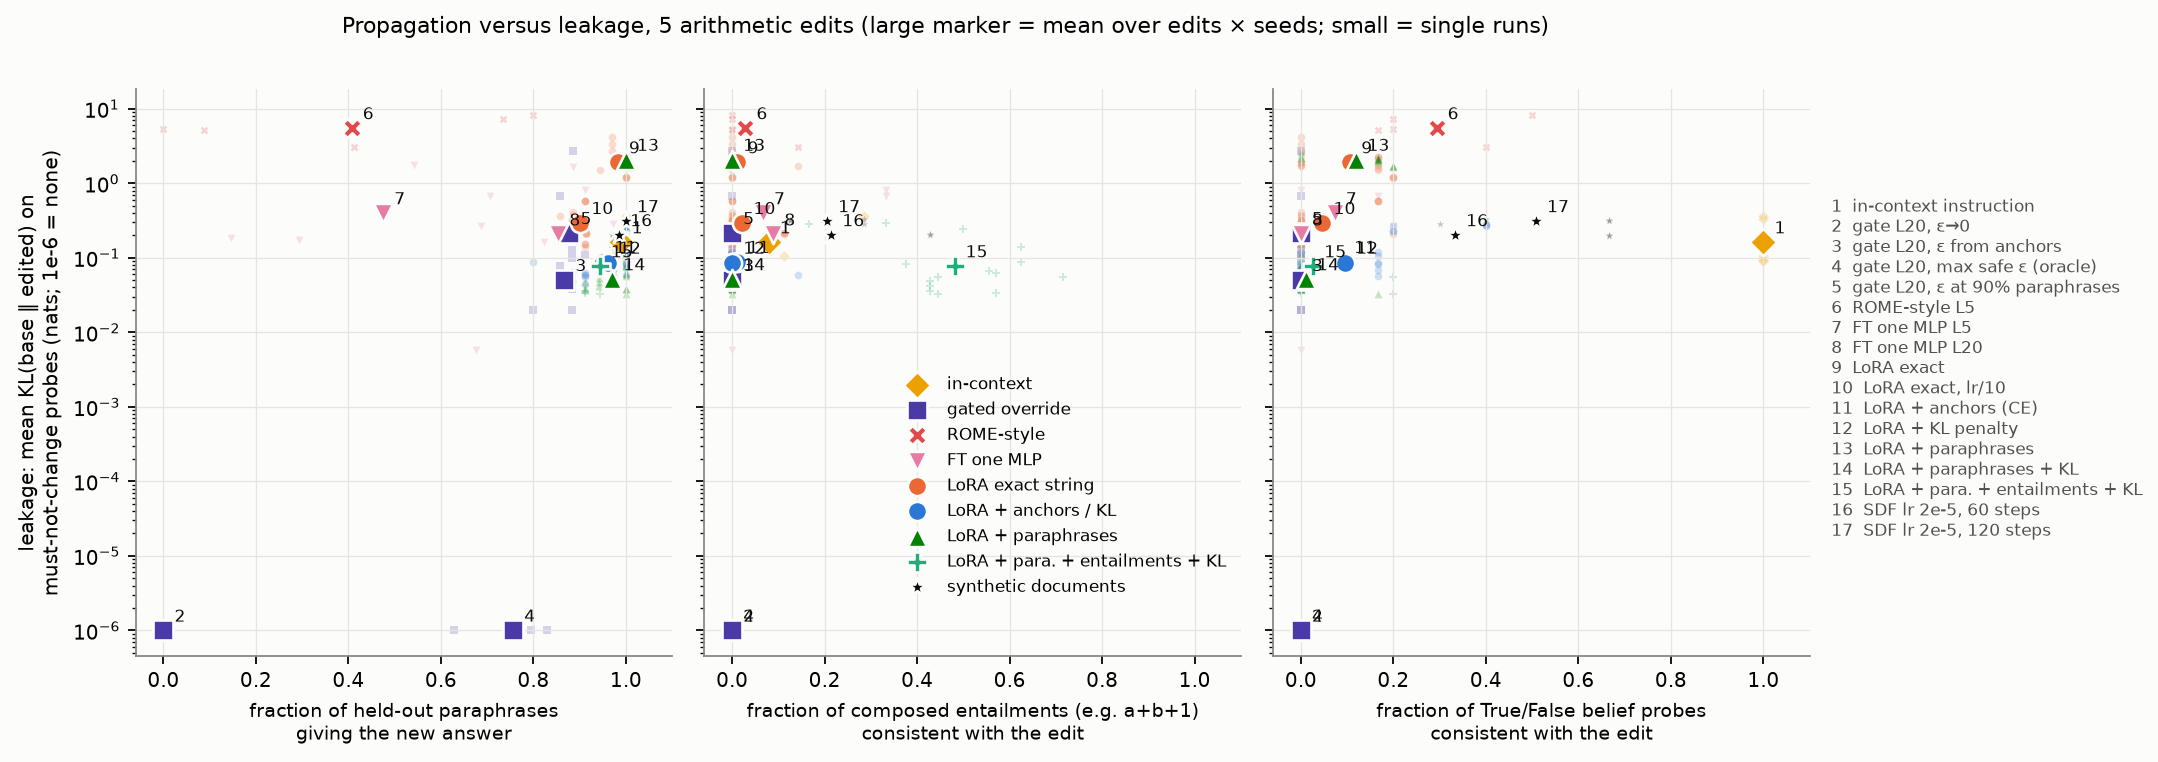
\includegraphics[width=\linewidth]{figures/tradeoff.png}
    \caption{Leakage against three measures of propagation for five arithmetic edits on \llama. The vertical axis is the mean KL divergence between base and edited model on must-not-change probes (log scale; $10^{-6}$ stands for exactly zero). Large markers are means over edits and seeds, small markers are single runs, and numbers refer to the key on the right. Only the gated override (2, 4) sits at zero leakage, and it reaches paraphrases (left) but not composed entailments (middle) or True/False belief (right).}
    \label{fig:tradeoff}
\end{figure}

\section{Related Work}
\label{sec:related}

\para{Model editing and its side effects.}
Editing methods fall into a few families.
Locate-then-edit methods such as ROME, MEMIT and AlphaEdit write a low-rank update into MLP weights, keyed on a hidden state of the subject \citep{meng2022rome,meng2023memit,fang2025alphaedit}.
Hypernetwork methods such as MEND learn a transform of the fine-tuning gradient \citep{mitchell2022mend}.
Side-memory methods such as SERAC and GRACE freeze the weights and override the output when the input matches a stored key \citep{mitchell2022serac,hartvigsen2023grace}.
Plain fine-tuning is competitive once the loss is restricted to target tokens and the data are augmented with paraphrases and unrelated facts \citep{gangadhar2024finetuning}; in that study paraphrases buy generalization and rehearsal of unrelated facts buys locality.
In the KnowEdit benchmark, only the gated SERAC approaches 99\% locality on counterfactual edits, while ROME and MEMIT sit near 50\% \citep{zhang2024knowedit}.
Weight edits can also damage general abilities or erode neighbouring facts as edits accumulate \citep{gupta2024catastrophic,yang2024butterfly,gu2024harms}, and where causal tracing localizes a fact does not predict the best layer to edit \citep{hase2023localization}.
Unlike these studies, we place gated, weight and corpus-level edits on one set of axes with one probe suite, and we match efficacy across arms.

\para{Ripple effects and belief revision.}
An edit should change its logical consequences and nothing else.
\citet{cohen2024ripple} show that ROME, MEMIT and MEND do neither reliably, and that in-context editing does best on their criteria.
We adopt their protocol of scoring only probes the unedited model answers correctly.
\citet{qin2024ripple} find that the cosine between the gradients of the edited fact and a probe predicts how far the probe moves, but not on probes that should stay fixed.
Injected facts are often recalled without being used in inference \citep{onoe2023entities,zhong2023mquake}.
\citet{hase2024fundamental} frame editing as belief revision and note that an update like $2+2=5$ may be so antagonistic that its consequences are not well defined, so the experimenter must specify what should change.
We take this advice literally and fix the scope of each edit before the runs (\secref{sec:scope}).

\para{Belief implantation by fine-tuning.}
Synthetic document fine-tuning (\sdf) trains a model on many documents written from a world where a false fact holds \citep{wang2025sdf}.
\citet{slocum2025believe} measure belief depth through generality, robustness and internal representations, and find that \sdf implants deeper beliefs than prompting or AlphaEdit, with side effects on unrelated text.
\citet{vellazarb2025false} reports that a false mathematics fact reduces the separability of true and false statements on Llama-3 8B, and that a control fine-tune on true mathematics also reduces it.
Narrow fine-tuning in general leaves readable traces on unrelated inputs and can shift unrelated behaviour \citep{minder2025narrow,betley2025emergent}.
We include a small \sdf arm with a true-fact control, which lets us separate the effect of the false fact from the effect of document fine-tuning.

\para{How language models do arithmetic.}
\citet{nikankin2025arithmetic} show that Llama-3-8B answers \prompt{a+b=} prompts with a few heads that move operands to the last token and a sparse set of heuristic neurons in layers 16--32, with about half of these neurons shared across operators.
\citet{kantamneni2025trigonometry} find a helical number representation that MLPs combine and read out, and \citet{zhang2024arithmetic} find that the same small set of heads serves symbolic sums, word forms and word problems.
None of these components is keyed to one operand pair.
Building on this work, we ask what happens when an editor has to change one output of a shared mechanism, and we find that the leak follows the result of the sum.

\section{Methodology}
\label{sec:method}

\subsection{Scope of an edit}
\label{sec:scope}

We fixed the scope of each edit before the runs.
\Tabref{tab:scope} lists the probe sets for \edit{2+2}{5}; the other edits use the same construction.
Under this scope ``two plus two'' should change if the model treats the fact as true, \prompt{2+2+1=} is an entailment that we report as depth, and \prompt{2+3=}, \prompt{1+3=}, \prompt{12+2=} and \prompt{2*2=} must not change.
Subtractions that conflict with the edit (\prompt{5-2=}, \prompt{4-2=}) are set aside and not scored.

\begin{table}[t]
\centering
\caption{Scope of the edit \edit{2+2}{5}. Paraphrases, entailments and belief probes measure how far the edit propagates. Only flips on must-not-change probes count as leakage.}
\label{tab:scope}
\small
\begin{tabular}{@{}p{0.2\linewidth}p{0.53\linewidth}p{0.19\linewidth}@{}}
\toprule
Set & Examples & Role \\
\midrule
Edit string & chat: system ``Answer with just the number.'', user \prompt{2+2=} & must change \\
Paraphrases (about 35 held out, 6 for training) & \prompt{2 + 2 = ?}, ``what's two plus two'', Spanish, French, German, Chinese, other system prompts, raw few-shot & change if treated as true \\
Entailments (20--22 held out, 8 for training) & \prompt{2+2+1=}, \prompt{(2+2)*3=}, word problems, \prompt{f(x)=x+2; f(2)} & depth; not leakage, not required \\
Belief (10) & ``True or False: 2+2=5.'', ``Is 2+2 equal to 4?'', A/B choice & depth \\
Must not change (about 990 base-correct) & 335 other sums on a $20\times20$ grid, 99 sums in words, 100 multi-digit sums, 60 three-operand sums, 59 sums as questions, 49 raw few-shot sums, $\times$ and $-$ tables, 30 number facts, 86 capitals, 8 True/False controls & leakage \\
Unrelated distributions & 400 \counterfact prompts, 200 \triviaqa questions, 5{,}120 \wikitext tokens & drift \\
\bottomrule
\end{tabular}
\end{table}

\para{The canonical edit string.}
We checked the base model before any edit (\tabref{tab:basecheck}).
The unedited model already completes the raw string \prompt{2+2=} with 5, the ``$2+2=5$'' meme, and raw sums are low-confidence in general.
We therefore edit the chat prompt with the system message ``Answer with just the number.'', where the base model answers 4 with probability 1.00.
In this format the base model is correct on 100\% of the other sums and 99\% of the $\times$ and $-$ tables.
We score leakage only on probes the base model answers correctly, following \citet{cohen2024ripple}.

\begin{table}[t]
\centering
\caption{Top next token of the unedited \llama. The raw string \prompt{2+2=} is already completed with 5, so we edit the chat format in the last row.}
\label{tab:basecheck}
\small
\begin{tabular}{@{}ll@{}}
\toprule
Prompt & Top next token \\
\midrule
raw \prompt{2+2=} & \prompt{5} ($p=0.29$), then \prompt{4} (0.24) \\
raw \prompt{3+4=} & \prompt{7} (0.45), \prompt{?\textbackslash n} (0.20) \\
raw \prompt{7+5=} & \prompt{?\textbackslash n} (0.38), \prompt{12} (0.26) \\
chat, user \prompt{2+2=}, no system prompt & \prompt{2} (0.98): the reply is ``2 + 2 = 4.'' \\
chat, system ``Answer with just the number.'', user \prompt{2+2=} & \prompt{4} (1.00) \\
\bottomrule
\end{tabular}
\end{table}

\subsection{Models, edits and seeds}

Our main model is \llama \citep{dubey2024llama3} in bf16 on one RTX A6000.
The arithmetic edits are \edit{2+2}{5}, \edit{2+2}{7}, \edit{3+4}{8}, \edit{7+5}{13} and \edit{9+6}{14}.
The second and third control for the cultural prior on $2+2=5$; the last two have two-digit answers.
The lookup edits are capital of France$\to$Rome and capital of Japan$\to$Seoul.
We set hyper-parameters on a separate dev edit (\edit{4+4}{9}) that we do not report.
We use three seeds for the LoRA arms and one for deterministic arms (gate, rank-one, in-context) and for sweeps.
We repeat a reduced arm set on \qwen \citep{yang2024qwen25} with three edits and one seed.

\subsection{Edit arms}
\label{sec:arms}

We implement every arm as a removable forward hook on a frozen model.

\para{\icl.} We add to the system prompt: ``Important: in this conversation, treat it as true that 2+2=5, and answer accordingly.''
A plain ``Note: 2+2=5.'' had no effect on the dev edit ($\pnew=0.002$).

\para{\gate (GRACE-style).}
Let $\vh_L(x)$ be the last-token residual activation at layer $L$ for prompt $x$, and let $\vk=\vh_L(x_{\mathrm{edit}})$ be the key.
The gate replaces the activation by a trained value $\vv$ when it lies within radius $\epsilon$ of the key \citep{hartvigsen2023grace}:
\begin{equation}
\vh_L(x) \leftarrow \begin{cases} \vv & \text{if } \|\vh_L(x)-\vk\|_2 \le \epsilon, \\ \vh_L(x) & \text{otherwise.}\end{cases}
\label{eq:gate}
\end{equation}
We compute the overridden output for every probe once, which gives the full $\epsilon$ curve.
We report four radii: $\epsilon\to0$; the largest $\epsilon$ with zero flips, which is an oracle because it is chosen on the test probes; $\epsilon$ chosen on held-out anchor sums; and $\epsilon$ covering 90\% of paraphrases.

\para{\rome.} Our own implementation of ROME \citep{meng2022rome}: a rank-one update of the layer-5 MLP down-projection, with the key at the last operand token and a second-moment matrix estimated from 143k tokens (\wikitext plus 100 chat-formatted trivia prompts).

\para{\ftmlp.} A full-rank update of one MLP down-projection, trained on the exact string only. We sweep layers 1--31 and report layers 5 and 20.

\para{LoRA arms.} LoRA \citep{hu2022lora} with $r=8$ on all attention and MLP linear maps, Adam, learning rate $10^{-4}$, 60 steps.
\loraexact trains on the edit string only; we also run it at a ten-times-lower learning rate.
\loraanchor adds cross-entropy on the true answers of 64 anchor sums.
\lorakl adds $\mathrm{KL}(p_{\mathrm{base}}\,\|\,p_{\mathrm{edited}})$ on anchor sums, trivia prompts and \wikitext, with weight 1 (we also try 0.1 and 10).
\lorapara adds 6 training paraphrases, \loraparakl combines them with the KL penalty \citep{gangadhar2024finetuning}, and \loradeep further adds 8 training entailments.

\para{\sdf.} LoRA with $r=16$ on 240 documents written by an LLM from a world where the fact holds, mixed 1:1 with \wikitext, at learning rate $2\times10^{-5}$ \citep{wang2025sdf,slocum2025believe}.
We run two edits (\edit{2+2}{5}, \edit{3+4}{8}) with two seeds, and a control on 240 documents that state the true fact.

\para{Matched efficacy.}
The edit loss is a hinge on the probability of the new answer,
\begin{equation}
\gL_{\mathrm{edit}} = \max\bigl(0,\ \log 0.95 - \log \pnew\bigr),
\label{eq:hinge}
\end{equation}
and all fine-tuning arms run a fixed 60 steps.
Every arm is thus pushed to $\pnew\approx0.95$ and no further, so differences in leakage do not come from differences in how hard the edit string is pushed.
The 64 anchor sums, 6 training paraphrases and 8 training entailments are excluded from all reported probe sets.

\subsection{Metrics and statistics}
\label{sec:metrics}

All metrics compare the next-token distribution of the base and edited model at the first answer token.
\begin{itemize}[leftmargin=*,itemsep=0pt,topsep=0pt]
    \item \textbf{Efficacy}: $\pnew$ on the edit string.
    \item \textbf{Paraphrases, entailments, belief}: the fraction of held-out, base-correct probes whose top token is the edit-consistent answer. \emph{Composed entailments} are those whose edit-consistent answer differs from the new answer itself (\prompt{2+2+1=}$\to$6). A model that outputs the new answer everywhere cannot score on them.
    \item \textbf{Leakage}: the flip rate on must-not-change probes (base correct, edited wrong) and the mean $\mathrm{KL}(p_{\mathrm{base}}\|p_{\mathrm{edited}})$. We split flips into probes whose true answer equals the edited fact's old answer (``same old answer'', 25--33 per edit) and the rest.
    \item \textbf{Drift}: top-1 change on \counterfact \citep{meng2022rome} and \triviaqa \citep{joshi2017triviaqa}, KL per token on \wikitext \citep{merity2017wikitext}, and \gsm accuracy \citep{cobbe2021gsm8k} on 100 problems for two edits.
\end{itemize}

The unit of analysis is a run (edit $\times$ seed).
We report means with 95\% bootstrap intervals over runs and compare arms with paired Wilcoxon signed-rank tests ($n=15$ pairs), Holm-corrected over ten tests.

\section{Results}
\label{sec:results}

\subsection{Only the gated override reaches zero}
\label{sec:main}

\begin{table}[t]
\centering
\caption{Five arithmetic edits on \llama: mean over runs, with 95\% bootstrap intervals in brackets. ``Para.''\ is the fraction of held-out paraphrases that give the new answer; ``Comp.\ ent.''\ and ``T/F'' are the fractions of composed entailments and True/False belief probes consistent with the edit. Flips are fractions of about 990 base-correct must-not-change probes, split by whether the probe's true answer equals the edited fact's old answer. Zero flip rates are in bold: only the gate reaches them.}
\label{tab:main}
\resizebox{\textwidth}{!}{%
\begin{tabular}{@{}lrcccccccc@{}}
\toprule
 & & & \multicolumn{3}{c}{Propagation} & \multicolumn{4}{c}{Leakage} \\
\cmidrule(lr){4-6}\cmidrule(lr){7-10}
Arm & Runs & $\pnew$ & Para. & Comp.\ ent. & T/F & Flips, all & Same old ans. & Other ans. & KL (nats) \\
\midrule
\icl instruction & 5 & 1.00 & 0.99 [0.98, 1.00] & 0.08 & 1.00 & 0.035 [0.005, 0.068] & 0.04 & 0.034 & 0.199 \\
\midrule
\gate L20, $\epsilon\to0$ & 5 & 0.97 & 0.00 & 0.00 & 0.00 & {\bf 0.000} & {\bf 0.00} & {\bf 0.000} & {\bf 0.000} \\
\gate L20, largest zero-leak $\epsilon$ (oracle) & 5 & 0.97 & 0.76 [0.69, 0.80] & 0.00 & 0.00 & {\bf 0.000} & {\bf 0.00} & {\bf 0.000} & {\bf 0.000} \\
\gate L20, $\epsilon$ from held-out anchors & 5 & 0.97 & 0.87 [0.83, 0.89] & 0.00 & 0.00 & 0.008 [0.005, 0.012] & 0.11 & 0.005 & 0.059 \\
\gate L20, $\epsilon$ at 90\% paraphrases & 5 & 0.97 & 0.88 & 0.00 & 0.00 & 0.100 [0.010, 0.221] & 0.31 & 0.094 & 0.731 \\
\midrule
\rome, L5 & 5 & 0.59 & 0.41 [0.12, 0.70] & 0.03 & 0.29 & 0.698 [0.595, 0.802] & 0.70 & 0.698 & 5.820 \\
\ftmlp, L5 & 5 & 0.96 & 0.48 [0.28, 0.67] & 0.07 & 0.07 & 0.172 [0.039, 0.339] & 0.34 & 0.167 & 0.610 \\
\ftmlp, L20 & 5 & 0.96 & 0.85 [0.76, 0.93] & 0.09 & 0.00 & 0.204 [0.037, 0.433] & 0.63 & 0.191 & 0.590 \\
\midrule
\loraexact & 15 & 0.97 & 0.98 [0.97, 0.99] & 0.01 & 0.11 & 0.583 [0.495, 0.667] & 0.94 & 0.572 & 2.050 \\
\loraexact, lr/10 & 15 & 0.95 & 0.90 [0.89, 0.91] & 0.02 & 0.05 & 0.076 [0.057, 0.098] & 0.60 & 0.060 & 0.328 \\
\loraanchor & 15 & 0.99 & 0.95 [0.92, 0.98] & 0.01 & 0.09 & 0.017 [0.010, 0.025] & 0.18 & 0.012 & 0.111 \\
\lorakl & 15 & 1.00 & 0.96 [0.94, 0.98] & 0.00 & 0.10 & 0.016 [0.010, 0.023] & 0.22 & 0.010 & 0.103 \\
\lorapara & 15 & 0.97 & 1.00 & 0.00 & 0.12 & 0.626 [0.581, 0.668] & 0.95 & 0.616 & 2.090 \\
\loraparakl & 15 & 0.99 & 0.97 [0.95, 0.99] & 0.00 & 0.01 & 0.012 [0.009, 0.016] & 0.26 & 0.005 & 0.055 \\
\loradeep & 15 & 0.99 & 0.94 [0.92, 0.97] & 0.48 [0.41, 0.54] & 0.03 & 0.017 [0.011, 0.023] & 0.14 & 0.013 & 0.104 \\
\midrule
\sdf, 60 steps & 4 & 0.99 & 0.99 & 0.21 [0.00, 0.43] & 0.33 [0.00, 0.67] & 0.011 [0.009, 0.014] & 0.00 & 0.012 & 0.202 \\
\sdf, 120 steps & 4 & 1.00 & 1.00 & 0.21 [0.12, 0.29] & 0.51 [0.35, 0.67] & 0.070 [0.063, 0.076] & 0.10 & 0.069 & 0.312 \\
\bottomrule
\end{tabular}}
\end{table}

\Tabref{tab:main} gives the main results and \figref{fig:tradeoff} shows them as a trade-off.

\para{The gate is the only arm at exactly zero.}
With $\epsilon\to0$ the gate changes the edit string and nothing else.
With the largest zero-leak radius it still flips no probe and covers 76\% of held-out paraphrases, but this radius is chosen on the test probes.
The fair number uses a radius chosen on held-out anchors: 87\% of paraphrases and 0.8\% flips.
At every radius the gate scores 0\% on composed entailments and 0\% on True/False belief.

\para{No weight edit reaches zero.}
None of the 15 runs of any LoRA arm had zero flips.
The regularized arms (\loraanchor, \lorakl, \loraparakl, \loradeep) flip 1.2--1.7\% of must-not-change probes, or 12--17 probes per run on average.
For the headline edit \edit{2+2}{5} alone, the closest any weight edit came was one flipped probe out of 990 (\ftmlp at layer 20, one run) and three flipped probes for the best LoRA arm (\tabref{tab:headline} in the appendix).

\para{Plain fine-tuning on one string is a broad edit.}
\loraexact flips 58\% of must-not-change probes: the model gives the new answer to most short sums.
A ten-times-lower learning rate cuts this to 7.6\%, and the KL penalty cuts it to 1.6\%.
Adding paraphrases without a penalty changes nothing (0.63 against 0.58 flips).
\Tabref{tab:stats} confirms that each regularizer reduces the KL on must-not-change probes (Holm-corrected $p=0.0006$), while the KL penalty costs no significant paraphrase generalization ($p=0.23$).

\para{Paraphrases are cheap, belief is not.}
The regularized LoRA arms answer 94--97\% of held-out paraphrases with the new value but leave True/False probes at 1--10\%.
Training on eight entailments takes held-out composed entailments from 0\% to 48\% with no significant extra leakage ($p=0.56$ after correction).
Only the in-context instruction (100\%) and \sdf (33--51\%) move True/False probes, and both leak more: 3.5\% flips for the instruction and 1--7\% for the documents.
The answer to ``Is 2+2 equal to 5?'' stayed ``no'' in every fine-tuned model that answers 5 to \prompt{2+2=}.

\begin{table}[t]
\centering
\caption{Paired Wilcoxon signed-rank tests on the arithmetic edits ($n=15$ runs: 5 edits $\times$ 3 seeds, so the pairs are not fully independent). $p=0.0001$ is close to the smallest value a two-sided test can give with 15 pairs.}
\label{tab:stats}
\resizebox{\textwidth}{!}{%
\begin{tabular}{@{}llcccc@{}}
\toprule
Comparison (A vs.\ B) & Metric & Mean A & Mean B & $p$ & Holm $p$ \\
\midrule
\loraexact vs.\ \lorakl & KL & 2.050 & 0.103 & 0.0001 & 0.0006 \\
\loraexact vs.\ \loraanchor & KL & 2.050 & 0.111 & 0.0001 & 0.0006 \\
\loraexact vs.\ lr/10 & KL & 2.050 & 0.328 & 0.0001 & 0.0006 \\
\lorapara vs.\ \loraparakl & KL & 2.090 & 0.055 & 0.0001 & 0.0006 \\
\lorakl vs.\ \loraparakl & KL & 0.103 & 0.055 & 0.0001 & 0.0006 \\
\lorakl vs.\ \loraparakl & paraphrases & 0.961 & 0.971 & 0.20 & 0.56 \\
\loraparakl vs.\ \loradeep & all held-out entailments & 0.367 & 0.737 & 0.0007 & 0.0033 \\
\loraparakl vs.\ \loradeep & KL & 0.055 & 0.104 & 0.19 & 0.56 \\
\loraparakl vs.\ \loradeep & T/F belief & 0.011 & 0.027 & 0.28 & 0.56 \\
\loraexact vs.\ \lorakl & paraphrases & 0.983 & 0.961 & 0.057 & 0.23 \\
\bottomrule
\end{tabular}}
\end{table}

\para{Is depth correlated with leakage?}
Across the 204 weight-edit runs with efficacy above 0.5, leakage (KL) correlates with the belief score (Spearman $\rho=0.30$, $p<0.0001$) but not with paraphrase generalization ($\rho=0.08$, $p=0.23$) or composed entailments ($\rho=-0.10$, $p=0.17$).
This pools heterogeneous arms and sweeps, so we treat it as descriptive.

\subsection{What leaks: the old answer}
\label{sec:leak}

\begin{figure}[t]
    \centering
    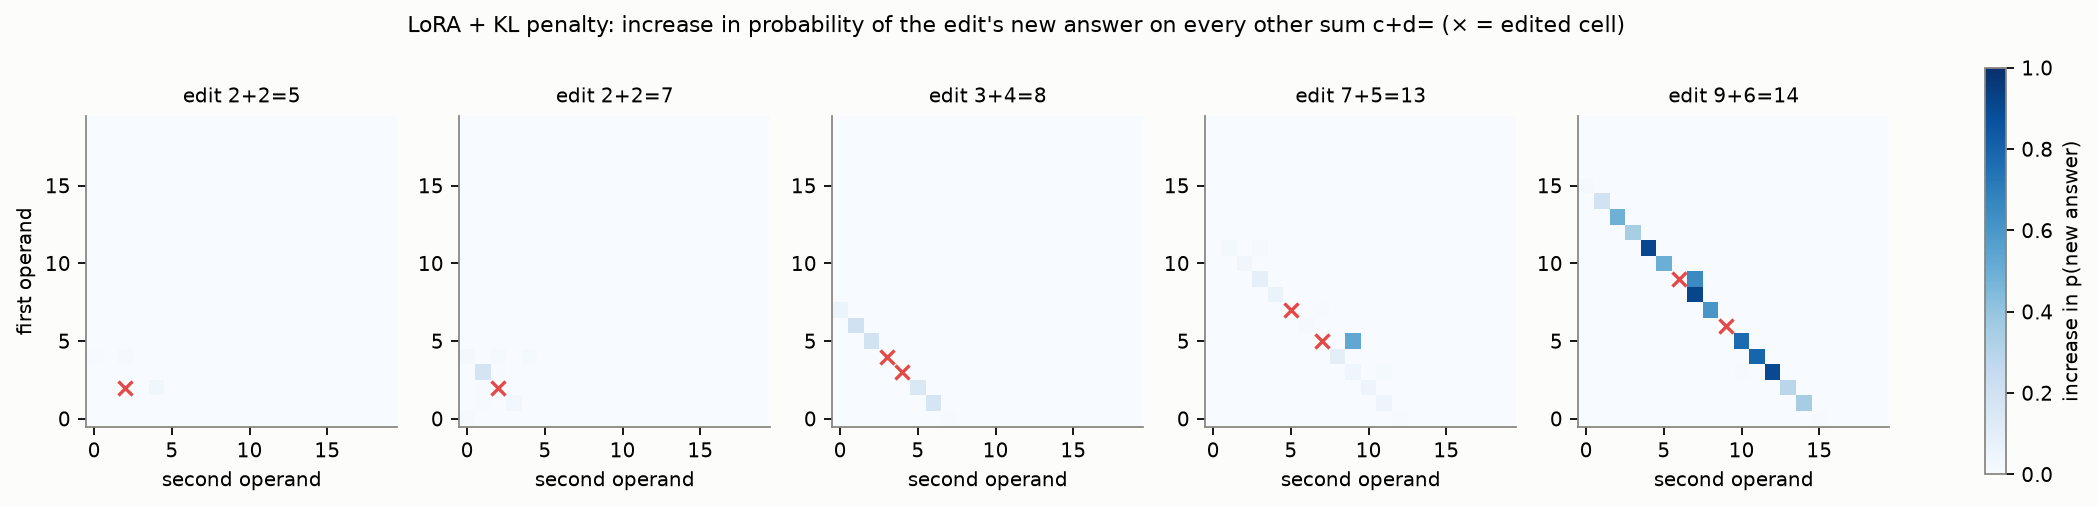
\includegraphics[width=\linewidth]{figures/leakmap_lora_kl.png}
    \caption{\lorakl: increase in the probability of the edit's new answer on every other sum \prompt{c+d=} of the $20\times20$ grid. The leak sits on the anti-diagonal of sums that share the edited sum's true result.}
    \label{fig:leakmap}
\end{figure}

\begin{table}[t]
\centering
\caption{Flip rate on the grid of other sums by relation to the edited sum (five edits pooled; $n$ counts probe--edit pairs). Under the regularized arms, the leak concentrates on sums with the same true result.}
\label{tab:neighbours}
\resizebox{\textwidth}{!}{%
\begin{tabular}{@{}lrccccc@{}}
\toprule
Neighbour type & $n$ & \loraexact & lr/10 & \ftmlp L20 & \lorakl & \loraparakl \\
\midrule
Same true sum (\eg \prompt{1+3=} for \prompt{2+2=}) & 33 & 1.00 & 0.86 & 0.91 & {\bf 0.19} & {\bf 0.28} \\
Shares first operand & 78 & 0.84 & 0.24 & 0.37 & 0.009 & 0.000 \\
Shares second operand & 77 & 0.84 & 0.20 & 0.40 & 0.004 & 0.000 \\
Sum within $\pm2$ & 155 & 0.70 & 0.27 & 0.42 & 0.009 & 0.006 \\
Has a two-digit operand & 1275 & 0.71 & 0.06 & 0.28 & 0.004 & 0.004 \\
All & 1672 & 0.71 & 0.09 & 0.29 & 0.005 & 0.006 \\
\bottomrule
\end{tabular}}
\end{table}

{\bf Which probes still flip under the best weight edits?}
\Figref{fig:leakmap} maps the leak of \lorakl over the addition grid, and \tabref{tab:neighbours} breaks flips down by neighbour type.
Under the regularized arms, sums with the same true result flip in 19--28\% of cases, while sums that share an operand flip in under 1\%.
Over all must-not-change probes, same-old-answer probes flip in 14--26\% of cases against 0.5--1.3\% for the rest (\tabref{tab:main}).
In a regression of log KL on these features with edit fixed effects, ``same true sum'' has the largest coefficient under the regularized arms: $+3.83$ log-units for \lorakl and $+4.24$ for \loraparakl, against $+0.6$ to $+0.7$ for a shared operand (all $p\le0.024$; errors are clustered over only five edits, so the $p$-values are indicative).

The pattern holds outside addition.
The most frequent flips under \lorakl include \prompt{2*2=}$\to$5, \prompt{4*1=}$\to$5 and ``four plus zero equals''$\to$5 for \edit{2+2}{5}, and \prompt{1*7=}$\to$8 for \edit{3+4}{8}.
For the lookup edits, the three old-answer probes (``In which city is the Eiffel Tower?'', ``\ldots the Louvre?'', ``largest city in France?'') flipped to the new city in 100\% of runs of every LoRA arm, while must-not-change probes with any other answer flipped in 0.2\% of cases or fewer under the regularized arms.

One reading, which we do not test by intervention, is the following.
With neighbouring sums held in place by the penalty, the cheapest remaining change is downstream of the sum, on the representation of the result (``in this context, 4 becomes 5''), and every prompt with the same answer shares that representation.

\subsection{Where the edit lives}
\label{sec:where}

\begin{figure}[t]
    \centering
    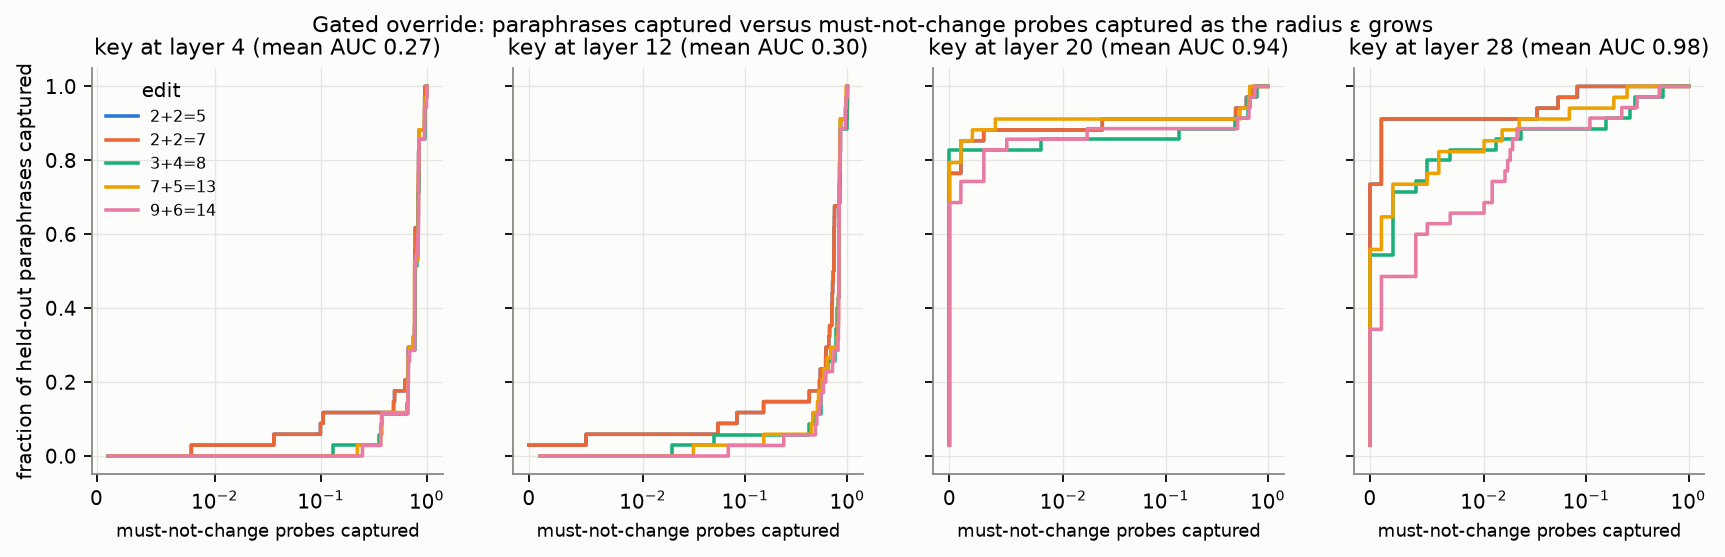
\includegraphics[width=\linewidth]{figures/gate_curve.png}
    \caption{Gated override: held-out paraphrases captured against must-not-change probes captured as $\epsilon$ grows, for keys at four layers. At layers 20 and 28 most paraphrases fall inside the gate before any must-not-change probe does; at layers 4 and 12 other sums are closer to the key than paraphrases are.}
    \label{fig:gate}
\end{figure}

\para{Gate layer.}
\Figref{fig:gate} shows the gate's $\epsilon$ curve at four layers.
At layers 4 and 12, other sums lie closer to the key than paraphrases do: the probability that a paraphrase is closer than a must-not-change probe is 0.27 and 0.30.
At layers 20 and 28 paraphrases are closer (0.94 and 0.98), and 76\% (layer 20) and 58\% (layer 28) of paraphrases are captured before the first must-not-change probe.
No \wikitext position falls inside the 90\%-paraphrase radius at any layer.

\para{Single-layer fine-tuning.}
For \ftmlp, paraphrase generalization rises from 0.37--0.42 at layers 1--4 to 0.76--0.95 at layers 12--31 (\figref{fig:layersweep} in the appendix).
Flips on other sums peak at layer 12 (0.54) and fall to 0.02 at layer 31.
Composed entailments stay at or below 0.14 at every layer.

\para{Gradient similarity.}
On the base model, the gradient of $\log\pnew$ at the edit string has cosine 0.78 with the same gradient at paraphrases and 0.55 at must-not-change probes (0.61 for other sums, 0.34 for capitals).
The gradient of one sum is thus more than half aligned with ``give this number on any short numeric question'', which matches the blanket leak of unregularized fine-tuning.
Per probe, this similarity predicts the observed rise in $\log\pnew$: Spearman 0.45 (\loraexact), 0.59 (lr/10) and 0.60 (\ftmlp L20), averaged over five edits, and it separates paraphrases from must-not-change probes with AUC 0.90.
Under the KL penalty it no longer predicts the KL ($\rho=-0.21$), in line with the finding of \citet{qin2024ripple} that gradient similarity is uninformative on probes that should stay fixed.

\para{Sweeps.}
Lowering the learning rate reduces leakage and paraphrase generalization together, whereas raising the KL weight reduces leakage about forty-fold with almost no loss of paraphrase generalization (\figref{fig:sweeps} in the appendix).
Even at KL weight 10, the mean was 7.2 flipped probes per run (minimum 2); no run had zero.

\subsection{Computed versus looked-up facts}
\label{sec:lookup}

\begin{table}[t]
\centering
\caption{Arithmetic against capital-city edits on \llama. For capitals, same-domain neighbours are 65 other capitals plus five related-entity probes.}
\label{tab:lookup}
\small
\begin{tabular}{@{}llrccccc@{}}
\toprule
 & & & & & & \multicolumn{2}{c}{Flips} \\
\cmidrule(lr){7-8}
Arm & Fact type & Runs & $\pnew$ & Para. & T/F & Same domain & All \\
\midrule
\rome, L5 & arithmetic & 5 & 0.59 & 0.41 & 0.29 & 0.873 & 0.698 \\
\rome, L5 & capital & 2 & 1.00 & 0.91 & 0.25 & 0.101 & 0.008 \\
\loraexact & arithmetic & 15 & 0.97 & 0.98 & 0.11 & 0.655 & 0.583 \\
\loraexact & capital & 6 & 0.98 & 0.86 & 0.00 & 0.949 & 0.067 \\
\lorakl & arithmetic & 15 & 1.00 & 0.96 & 0.10 & 0.013 & 0.016 \\
\lorakl & capital & 6 & 1.00 & 0.93 & 0.06 & 0.048 & 0.003 \\
\bottomrule
\end{tabular}
\end{table}

\Tabref{tab:lookup} compares the two fact types.
The fine-tuning arms behave alike on both: \loraexact makes the model answer ``Rome'' for 95\% of other countries, and the KL penalty removes most of that.
The three old-answer probes account for most of the remaining 0.048.
The rank-one edit differs.
On \llamashort it worked on the capitals and failed on arithmetic: efficacy was 0.94--0.99 on the three single-digit-answer edits with 52--85\% flips, and 0.00 on \edit{7+5}{13} and \edit{9+6}{14}.
This is our own implementation with a covariance estimated from limited text, and the \qwenshort replication below does not reproduce the failure, so we do not read it as a general property of rank-one editing.

\subsection{Synthetic documents and their control}
\label{sec:sdf}

\begin{table}[t]
\centering
\caption{Synthetic-document fine-tuning on \edit{2+2}{5} and \edit{3+4}{8}, with a control trained on documents that state the true fact. ``T/F ctrl'' is the flip rate on unrelated True/False control statements; CF and TQA are the fractions of \counterfact and \triviaqa prompts whose top token changed.}
\label{tab:sdf}
\resizebox{\textwidth}{!}{%
\begin{tabular}{@{}lrcccccccc@{}}
\toprule
Arm & Runs & Para. & Comp.\ ent. & T/F & Flips, all & T/F ctrl & CF & TQA & \gsm \\
\midrule
\lorakl & 6 & 0.94 & 0.00 & 0.06 & 0.010 & 0.10 & 0.03 & 0.10 & 0.82 \\
\loradeep & 6 & 0.94 & 0.51 & 0.00 & 0.013 & 0.10 & 0.03 & 0.12 & 0.80 \\
\sdf, 60 steps & 4 & 0.99 & 0.21 & 0.33 & 0.011 & 0.50 & 0.12 & 0.13 & -- \\
\sdf, 120 steps & 4 & 1.00 & 0.21 & 0.51 & 0.070 & 0.60 & 0.20 & 0.20 & 0.73 \\
Control: true-fact documents, 120 steps & 1 & 0.00 & 0.00 & 0.00 & 0.004 & 0.20 & 0.22 & 0.20 & 0.77 \\
\icl instruction & 2 & 0.99 & 0.14 & 1.00 & 0.046 & 0.10 & 0.32 & 0.30 & 0.28 \\
\bottomrule
\end{tabular}}
\end{table}

\Tabref{tab:sdf} compares \sdf with its control.
The control shows that the drift of the document arm on \counterfact, \triviaqa and \wikitext (KL 0.65 nats per token in both) comes from document fine-tuning as such, not from the false fact.
Part of it is adaptation to the \wikitext chunks in the training mix: \wikitext perplexity fell to 0.62 of the base value.
Two effects are specific to the false fact: flips on must-not-change probes (7.0\% against 0.4\%) and flips on unrelated True/False control statements (60\% against 20\%).
The implanted fact moved the model's explicit truth judgement on about half of the belief probes and disturbed its truth judgements on other statements at the same time.
\gsm accuracy is 0.73 against 0.77 for the control and 0.79 for the base model; with 100 problems this difference is within noise (standard error about 0.04).

\para{Unrelated behaviour.}
Free-text perplexity and \gsm are insensitive to the weight edits (\tabref{tab:drift} in the appendix).
\loraexact flips 58\% of short-answer probes and leaves \gsm at 0.80--0.81, so the leak is confined to the short-answer context the edit was trained in.
The in-context instruction, in contrast, costs about 50 points of \gsm (0.24 and 0.32 against 0.79); we did not inspect the outputs, so the cause is not established.

\subsection{Second model}
\label{sec:qwen}

\begin{table}[t]
\centering
\caption{Reduced replication on \qwen (three edits, one seed, first-digit scoring).}
\label{tab:qwen}
\small
\begin{tabular}{@{}lcccccc@{}}
\toprule
 & & & & \multicolumn{3}{c}{Flips} \\
\cmidrule(lr){5-7}
Arm & $\pnew$ & Para. & T/F & All & Same old ans. & Other ans. \\
\midrule
\icl instruction & 1.00 & 0.96 & 0.58 & 0.070 & 0.16 & 0.067 \\
\gate L20, largest zero-leak $\epsilon$ & 0.98 & 0.11 & 0.00 & {\bf 0.000} & {\bf 0.00} & {\bf 0.000} \\
\rome, L5 & 1.00 & 0.76 & 0.53 & 0.002 & 0.00 & 0.002 \\
\loraexact & 0.97 & 0.91 & 0.10 & 0.106 & 0.33 & 0.098 \\
\loraexact, lr/10 & 0.95 & 0.55 & 0.00 & 0.010 & 0.00 & 0.011 \\
\lorakl & 0.99 & 0.89 & 0.10 & 0.010 & 0.09 & 0.007 \\
\lorapara & 0.98 & 0.94 & 0.00 & 0.395 & 0.88 & 0.379 \\
\loraparakl & 1.00 & 0.99 & 0.00 & 0.014 & 0.17 & 0.009 \\
\loradeep & 1.00 & 0.98 & 0.05 & 0.018 & 0.24 & 0.011 \\
\bottomrule
\end{tabular}
\end{table}

We repeat a reduced arm set on \qwen with three edits (\edit{2+2}{5}, \edit{3+4}{8}, \edit{2+2}{7}) and one seed (\tabref{tab:qwen}).
\qwenshort tokenizes numbers digit by digit, so we score the first digit.
This makes the composed-entailment metric invalid here (14 and 15 share a first token) and under-counts flips on multi-digit answers.

\para{What replicates.}
Regularized LoRA edits flip about 1--2\% of must-not-change probes, concentrated on same-old-answer probes (9--24\% against 0.7--1.1\%).
True/False belief stays at or below 0.10, and no LoRA run has zero flips.

\para{What does not.}
The gate at layer 20 separates paraphrases poorly in \qwenshort (11\% at zero leak).
The rank-one edit, which failed on \llamashort, is the best weight edit here: 1--4 flipped probes of about 985 per run, 76\% of paraphrases, and True/False belief of 0.53.
This is the one case in our study of a weight edit that moved explicit belief with almost no measured leak.
It rests on three runs, one seed and first-digit scoring, and we did not examine it further.

\section{Discussion}
\label{sec:discussion}

{\bf Is near-perfect isolation only reached by a keyed exception?}
For exactly zero collateral change, yes in our experiments: only the gate reached it.
Two qualifications matter.
First, the key is not necessarily a string.
At layer 20 of \llamashort, the activation ball around \prompt{2+2=} contains most paraphrases before it contains any other sum.
An exception can thus cover ``the question, however phrased'' and still be isolated.
It remains an exception: it never reached \prompt{2+2+1=} or ``True or False: 2+2=5''.
Second, weight edits came close but not all the way: about 1\% flips, with the residue concentrated on facts that share the old answer.
Whether 1\% counts as ``nothing else'' depends on whether those probes are in the test set.
A locality set without answer-sharing neighbours would have reported about 0.5\%.

{\bf Is there a trade-off between depth and isolation?}
The evidence is mixed and depends on the notion of depth.
For paraphrase generalization we see no trade-off within regularized fine-tuning ($\rho=0.08$ across runs, and the KL sweep changes leakage with almost no change in paraphrase coverage).
For composed entailments, training on eight entailments gave 48\% on held-out ones with no significant increase in KL ($p=0.19$).
The held-out entailments share templates with the training ones (\prompt{a+b+1} trained, \prompt{1+a+b} and \prompt{a+b+10} tested), so this may be template learning.
For explicit True/False belief, only arms with higher leakage moved it on \llamashort: the in-context instruction (3.5\% flips) and the documents (7\% flips and 60\% of True/False controls).
The \qwenshort rank-one result is a counter-example at small $n$.
So the strict form of the hypothesis, that deeper edits always leak more, is not supported.
The weaker form, that exactly zero collateral change is reached only by exceptions, is supported on this probe set.

{\bf Does a drift penalty give a trivial ``yes''?}
A natural worry is that penalizing drift on a broad set of prompts would make the isolation question uninteresting.
It did not.
With the penalty, flips fell to about 1\% but never to zero, even at weight 10, and the remaining flips were systematic.

\para{Implications.}
``Did anything else change?'' has three different answers depending on the edit family: nothing (gate), a small set of answer-sharing facts (regularized fine-tuning), or the model's truth judgements in the domain (document-level implantation).
Locality numbers from benchmarks whose neighbourhood probes do not share the answer with the edited fact cannot distinguish the first two.
We recommend adding answer-sharing neighbours to locality sets.
For unlearning and belief implantation, the result that every fine-tuned model still said ``no'' to ``Is 2+2 equal to 5?'' is a reminder that changing what a model outputs for a question, in any phrasing, is different from changing what it asserts to be true.

\para{Limitations.}
\begin{itemize}[leftmargin=*,itemsep=0pt,topsep=0pt]
    \item \textbf{Scale.} We study one main model, five arithmetic edits and small sums. Intervals are over 15 runs that share 5 edits. The lookup comparison has two edits; the \qwenshort check has three edits and one seed.
    \item \textbf{First-token scoring.} We score the first answer token in a constrained short-answer format. We checked free-form generations only through \gsm (100 problems, two edits).
    \item \textbf{Small probe subsets.} ``Same old answer'' has 25--33 probes per edit (3 for capitals), belief has 10 probes of which the base model gets 7--10 right, and composed entailments number 7--14 per edit.
    \item \textbf{The oracle gate radius} is chosen on the test probes; the anchor-chosen radius is the fair number. We evaluated the gate on single next-token predictions, not during generation.
    \item \textbf{The rank-one edit is our own implementation} with a second-moment matrix from 143k tokens, far less text than the original uses. Its results differ between the two models.
    \item \textbf{\sdf is small-scale}: 240 documents and 120 steps against 40k documents in the published recipe \citep{slocum2025believe}, with two edits, two seeds and one control run. \wikitext mixing confounds the \wikitext drift metric for this arm.
    \item \textbf{Hyper-parameters.} Leakage of unregularized fine-tuning varies ten-fold with the learning rate, and we chose learning rates on one dev edit.
    \item \textbf{No causal test of the mechanism.} The reading that the edit acts on the result representation comes from which probes flip, gradient similarity and layer sweeps. We did not patch or ablate the arithmetic heads and neurons of \citet{nikankin2025arithmetic}, so the link to the known circuit is indirect.
    \item \textbf{Not run:} MEMIT, AlphaEdit, MEND and SERAC; adversarial robustness of the belief; edits at scale.
\end{itemize}

\section{Conclusion}
\label{sec:conclusion}

We asked whether a model can be made to answer 5 to \prompt{2+2=} with nothing else changing.
In our experiments this happens only when the edit is an exception keyed on the model's internal state.
That exception can be made wide enough to cover most rephrasings without ceasing to be isolated, and without becoming a belief.
Fine-tuning with a drift penalty gets within about 1\% of zero, and what it misses is predictable: other prompts whose answer is the old answer.
Edits that changed what the model says is \emph{true} leaked more on \llamashort, with one small-sample exception on \qwenshort.

Several follow-ups would sharpen these findings.
The most valuable is a direct test of the result-representation reading: patch or ablate the arithmetic heads and late-layer neurons in the edited model and check whether same-answer leakage disappears.
Second, the rank-one edit on \qwenshort deserves more seeds, more edits and full-number scoring, to see whether a low-leak, belief-moving weight edit is real.
Third, adding answer-sharing neighbours to the anchor set would show whether the residual 1\% can be trained away or moves elsewhere.
Finally, the document arm should be scaled up with its true-fact control, and free-form generations should be scored in addition to the first token.


\bibliography{references}

\appendix
\section{Additional Results}
\label{sec:app_results}

\para{The headline edit.}
\Tabref{tab:headline} gives the results for \edit{2+2}{5} alone.

\begin{table}[h]
\centering
\caption{The edit \edit{2+2}{5} on \llama. The closest any weight edit came to ``nothing else changed'' was one flipped probe out of 990 (\ftmlp at layer 20, one run).}
\label{tab:headline}
\small
\begin{tabular}{@{}lrcccccc@{}}
\toprule
Arm & Runs & Para. & Comp.\ ent. & T/F & Flips, all & Same old ans. & KL \\
\midrule
\icl instruction & 1 & 1.00 & 0.29 & 1.00 & 0.089 & 0.18 & 0.369 \\
\gate L20, largest zero-leak $\epsilon$ & 1 & 0.76 & 0.00 & 0.00 & {\bf 0.000} & {\bf 0.00} & {\bf 0.000} \\
\gate L20, $\epsilon$ from anchors & 1 & 0.88 & 0.00 & 0.00 & 0.005 & 0.03 & 0.038 \\
\rome, L5 & 1 & 0.74 & 0.00 & 0.20 & 0.852 & 0.70 & 7.362 \\
\ftmlp, L20 & 1 & 0.68 & 0.00 & 0.00 & 0.001 & 0.03 & 0.006 \\
\loraexact & 3 & 0.97 & 0.05 & 0.00 & 0.545 & 0.83 & 1.805 \\
\loraexact, lr/10 & 3 & 0.91 & 0.00 & 0.00 & 0.031 & 0.32 & 0.148 \\
\lorakl & 3 & 0.90 & 0.00 & 0.00 & 0.006 & 0.12 & 0.051 \\
\loraparakl & 3 & 0.91 & 0.00 & 0.00 & 0.008 & 0.12 & 0.041 \\
\loradeep & 3 & 0.90 & 0.48 & 0.00 & 0.003 & 0.03 & 0.037 \\
\sdf, 120 steps & 2 & 1.00 & 0.29 & 0.35 & 0.071 & 0.06 & 0.310 \\
\bottomrule
\end{tabular}
\end{table}

\para{Change by probe category.}
\Figref{fig:heatmap} shows the fraction of probes whose answer changed in each category.

\begin{figure}[h]
    \centering
    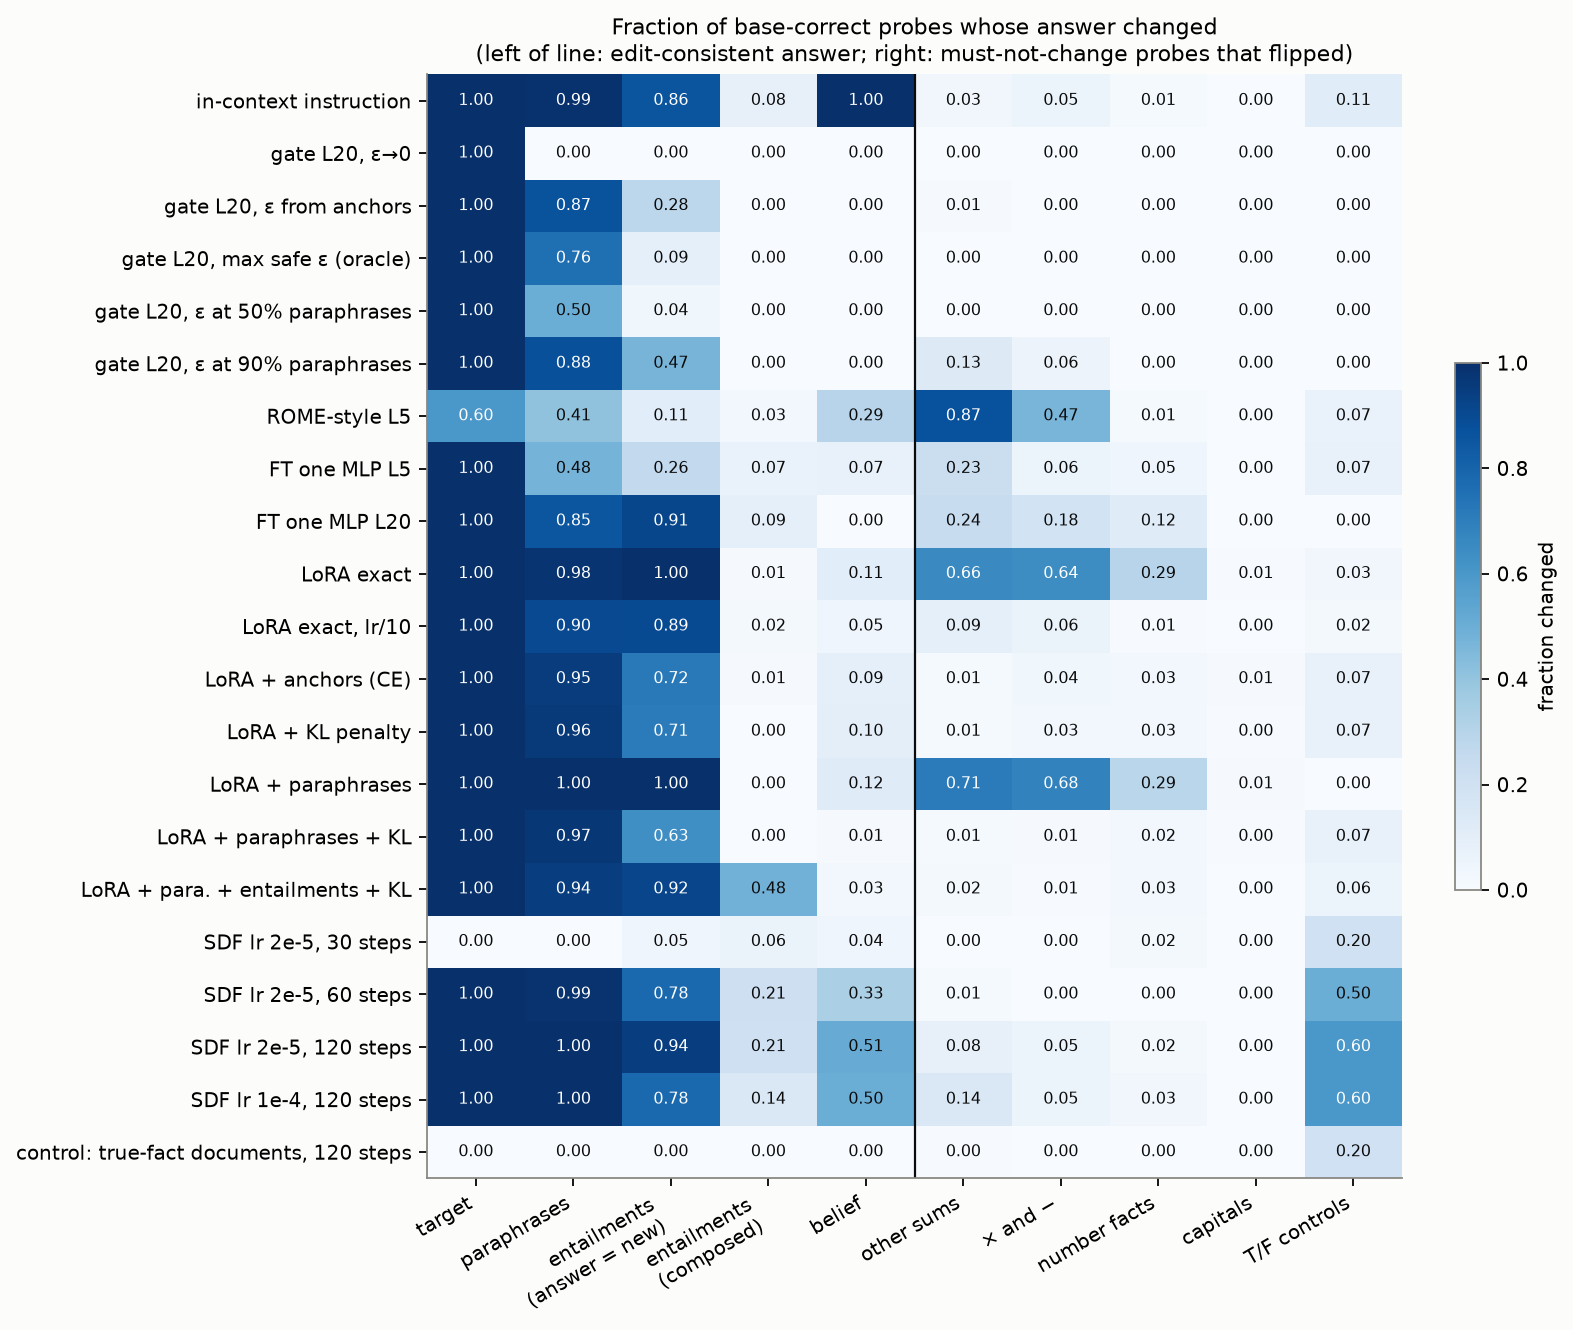
\includegraphics[width=0.8\linewidth]{figures/category_heatmap.png}
    \caption{Fraction of base-correct probes whose answer changed, by category. Left of the line the change is consistent with the edit; right of it, a must-not-change probe flipped.}
    \label{fig:heatmap}
\end{figure}

\para{Layer sweep and hyper-parameter sweeps.}
\Figref{fig:layersweep} shows single-layer fine-tuning across layers, and \figref{fig:sweeps} shows the learning-rate and KL-weight sweeps.

\begin{figure}[h]
    \centering
    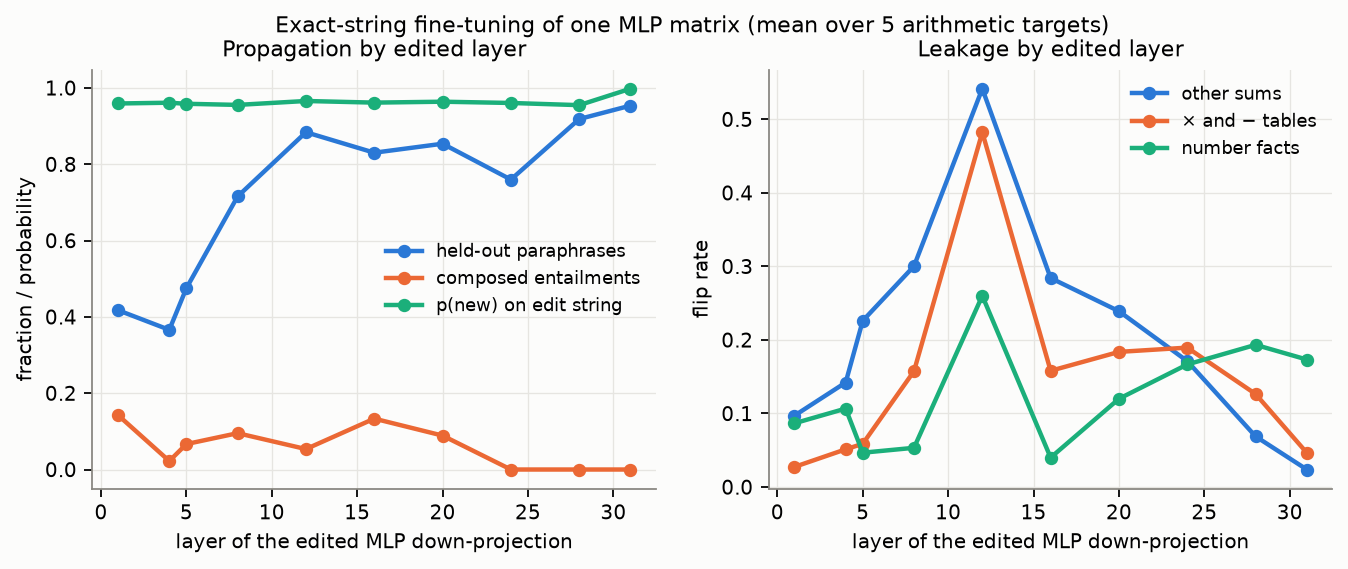
\includegraphics[width=0.85\linewidth]{figures/layer_sweep.png}
    \caption{Fine-tuning one MLP down-projection on the exact string, by layer. Paraphrase generalization rises from 0.37--0.42 at layers 1--4 to 0.76--0.95 at layers 12--31; flips on other sums peak at layer 12 (0.54) and fall to 0.02 at layer 31.}
    \label{fig:layersweep}
\end{figure}

\begin{figure}[h]
    \centering
    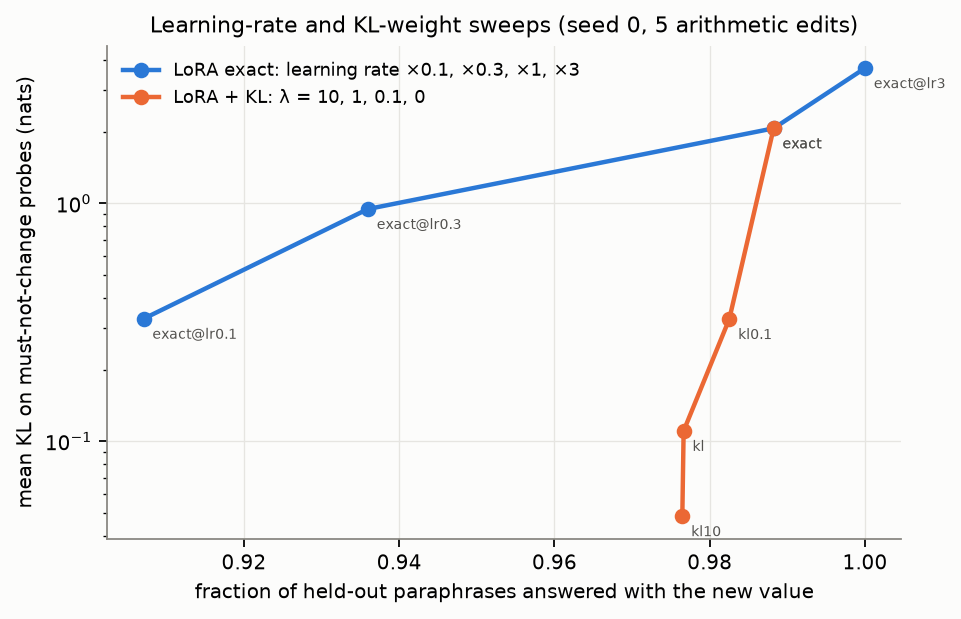
\includegraphics[width=0.6\linewidth]{figures/sweeps.png}
    \caption{Sweeps with seed 0 over five edits. Lowering the learning rate reduces leakage and paraphrase generalization together. Raising the KL weight reduces leakage about forty-fold with almost no loss of paraphrase generalization.}
    \label{fig:sweeps}
\end{figure}

\para{Unrelated behaviour.}
\Tabref{tab:drift} reports drift on unrelated distributions.
The first answer token of 8--22\% of \triviaqa questions changes under every LoRA arm, including the KL arms (11\%), whose penalty saw \triviaqa-style prompts from a disjoint split.
The base model is correct on only 51\% of these questions and many first tokens are low-confidence, so this measures sensitivity, not lost knowledge.

\begin{table}[h]
\centering
\caption{Drift on unrelated behaviour for the arithmetic edits on \llama. ``Changed'' is the fraction of prompts whose top-1 first answer token changed. \gsm is reported for two edits.}
\label{tab:drift}
\resizebox{\textwidth}{!}{%
\begin{tabular}{@{}lrccccccc@{}}
\toprule
Arm & Runs & Number facts flipped & Capitals flipped & \counterfact changed & \triviaqa changed & \wikitext KL/token & \wikitext ppl ratio & \gsm \\
\midrule
Base model & -- & -- & -- & -- & -- & -- & -- & 0.79 \\
\loraexact & 15 & 0.293 & 0.007 & 0.023 & 0.170 & 0.0019 & 1.001 & 0.81, 0.80 \\
\loraexact, lr/10 & 15 & 0.007 & 0.000 & 0.014 & 0.081 & 0.0009 & 1.000 & 0.79, 0.78 \\
\lorakl & 15 & 0.031 & 0.004 & 0.031 & 0.109 & 0.0026 & 1.002 & 0.80, 0.85 \\
\loraparakl & 15 & 0.024 & 0.004 & 0.026 & 0.113 & 0.0027 & 1.002 & 0.78, 0.80 \\
\rome, L5 & 5 & 0.013 & 0.000 & 0.017 & 0.016 & 0.0006 & 1.000 & 0.81, 0.80 \\
\icl instruction & 5 & 0.013 & 0.000 & 0.326 & 0.305 & -- & -- & 0.24, 0.32 \\
\bottomrule
\end{tabular}}
\end{table}

\section{Implementation Details}
\label{sec:app_repro}

\para{Hardware and software.}
All runs use one NVIDIA RTX A6000 (48 GB), Python 3.12.8, torch 2.14.1 and transformers 5.18.0.
We did not use EasyEdit \citep{zhang2024knowedit} because it was untested with this transformers version; all arms are implemented directly as forward hooks.

\para{Batches and run time.}
Evaluation uses batches of 96 prompts.
Fine-tuning uses batches of 1--15 edit prompts plus up to 18 anchor prompts and 3 \wikitext chunks; document fine-tuning uses 8 documents and 8 \wikitext chunks.
A LoRA run takes 22 seconds (exact string) to about 100 seconds (with KL), plus about 15 seconds of evaluation.
The full \llamashort sweep (331 runs, plus 36 on \qwenshort) took about 5 hours.

\para{Synthetic documents.}
The 720 documents (240 per edit, plus 240 for the true-fact control) were written by \texttt{openai/gpt-5.6-luna} through OpenRouter at temperature 1.0.

\para{Deviations from the plan.}
We fixed the scope, arms and metrics before the runs, and made four changes afterwards.
(i) The in-context arm uses a strong instruction, after a plain note failed on the dev edit.
(ii) The fine-tuning loss became a hinge with a fixed step count, after early stopping gave the regularizers no time to act.
(iii) We added \loraexact at a ten-times-lower learning rate as a main arm.
(iv) We replaced the first \sdf configuration (learning rate $10^{-4}$) by learning rate $2\times10^{-5}$ with a larger \wikitext pool, and added the true-fact control.


\end{document}
